% Chapter 1
\chapter{Marco Teórico} % Main chapter title

\label{Cap_SDT} % For referencing the chapter elsewhere, use \ref{Chapter1} 

%----------------------------------------------------------------------------------------

% Define some commands to keep the formatting separated from the content 
\newcommand{\keyword}[1]{\textbf{#1}}
\newcommand{\tabhead}[1]{\textbf{#1}}
\newcommand{\code}[1]{\texttt{#1}}
\newcommand{\file}[1]{\texttt{\bfseries#1}}
\newcommand{\option}[1]{\texttt{\itshape#1}}

%----------------------------------------------------------------------------------------

\section{Teoría de Detección de Señales}

%Detectar ciertos estados en el mundo es importante para guiar nuestro comportamiento
Uno de los problemas más frecuentes a los que se enfrentan los organismos como sistemas inmersos en entornos variables que buscan optimizar su comportamiento, es la detección de estados o eventos específicos -señales- que de acuerdo a su experiencia y tras la definición de ciertas relaciones de contingencia, les proporcionen información relevante sobre el estado del mundo, las restricciones vigentes y la disponibilidad de eventos biológicamente importantes, \parencite{McNicol1}.\\

%Origen y expansión de la Teoría de Detección de Señales en la psicología y otras áreas
La Teoría de Detección de Señales (TDS o SDT, por sus siglas en inglés) aparece por primera vez en 1954 -como tantos otros avances científicos y tecnológicos motivados por las necesidades planteadas por la Segunda Guerra Mundial- en el contexto del estudio y desarrollo de radares para detectar señales eléctricas específicas \parencite{Peterson1954}. Muy poco tiempo después, los psicólogos John A. Swets y Wilson P. Tanner contribuyeron a la expansión de la teoría a un contexto psicológico, como un modelo para estudiar la percepción de los organismos, \parencite{Tanner1954, Swets1961}. Desde entonces, la TDS constituye uno de los modelos más estudiados, desarrollados y ampliamente aplicados en Psicología \parencite{Stainslaw1999}, extendiéndose desde su foco inicial en el estudio de la percepción \parencite{Rosenholtz2001, Pessoa2005, Wallis2007} hacia el estudio de cualquier fenómeno o tarea donde los organismos se enfrenten al problema de emitir -y guiar su comportamiento en función a- juicios de detección; por ejemplo, en materia de la emisión de diagnósticos clínicos \parencite{Grossberg1978, Swets2000, Boutis2010}, en el estudio de ciertas condiciones clínicas \parencite{Westermann2010, Bonnel2003, Brown1994, Naliboff1981}, en el estudio de la identificación visual de testigos \parencite{Gronlund2014, Wixted2014, Wixted2016} y un muy amplio 'etcétera' \parencite{Gordon1974, Nuechterlein1983, Harvey1992, Verghese2001}.\\ 

%La Teoría de Detección de señales como un modelo descriptivo para el problema de la detección que admite la importancia de la incertidumbre, como parte del entorno y como motor en el uso de sesgos de respuesta.
La TDS constituye un modelo estadístico que describe el problema al que se enfrentan los organismos inmersos en situaciones de detección en ambientes con incertidumbre, donde las señales -los estímulos cuya ocurrencia interesa detectar- coexisten con ruido -estímulos que no son la señal pero que pueden confundirse con esta-. Se trata de un modelo de decisión que entiende la detección como una tarea de elección, donde los organismos no responden simplemente con base en lo que perciben, sino que eligen el juicio de detección que les permita guiar su comportamiento de la manera mas óptima posible dada la información que poseen y la evidencia presente, \parencite{Swets2000, Killeen2014}.\\

La generalizabilidad del modelo de la TDS al estudio de distintos fenómenos y tareas de detección se debe a lo abstracto de sus elementos: la 'señal' que interesa detectar puede ser desde un estímulo concreto -una luz o un tono- hasta la pertenencia a una categoría -una enfermedad o amenaza- y el 'ruido' es simplemente todo elemento presente en el entorno de la tarea que no sea la señal, \parencite{Stainslaw1999, McNicol1}.\\ 

\subsection{Supuestos generales del modelo}

%La TDS distingue dos grandes factores en la emisión de un juicio o respuesta: La discriminabilidad y el sesgo.
La TDS funciona como una herramienta -o marco de análisis- para traducir el desempeño observado en tareas de detección en inferencias sobre la precisión con que la señal se distingue del ruido (la discriminabilidad) y la posible preferencia -o tendencia- del sistema detector a responder en favor o en contra de esta (el sesgo), \parencite{McNicol1}. Esta distinción entre la Discriminabilidad de los estímulos comprometidos y el Sesgo del sistema, como factores que interactúan en la emisión de juicios de detección, es una de las principales propiedades de la TDS \parencite{Swets1961} cuya importancia e implicaciones se discuten a continuación:\\

\textbf{1.- El papel de la Discriminabilidad: Siempre hay incertidumbre}\\

%Hay variabilidad en todos los estímulos implicados en las tareas de detección (en la señal y en los estímulos no-señal)
Se habla de la detección de señales como un problema de adaptación porque se asume que la variabilidad en la presentación y percepción de los estímulos en el ambiente merma la capacidad de los organismos de emitir juicios de detección que reflejen el estado del mundo con certeza, \parencite{Tanner1954}. Y dado que los estímulos-señal coexisten en el mundo con estímulos-ruido, saber qué tan salientes son las señales respecto del ruido es uno de los factores más importantes para determinar qué tan difícil es su detección para los organismos. En términos de la TDS, se habla de dicha dificultad como 'la discriminabilidad' de los estímulos comprometidos en la tarea.\\

De acuerdo con la TDS, la discriminabilidad constituye el primer gran componente en la emisión de juicios de detección óptimos que reflejen el verdadero estado del mundo y permitan al organismo actuar conforme a las consecuencias vigetes. Suele explicarse en términos de:\\ %  1) la variabilidad intrínseca en la presentación de las señales y 2) el ruido con que ésta coexiste.\\

\underline{a) La Variabilidad en la Señal}\\

%Existe variabilidad en la forma en que percibimos los estímulos que nos rodean. Los sistemas sensoriales y perceptuales se comportan como instrumentos de medición (error de medida)
La noción de variabilidad ha sido uno de los principales motores para el desarrollo de modelos estadísticos en Psicología. Desde que Fechner extendiera las ideas planteadas por Gauss sobre la incertidumbre contenida en toda medición -la idea de que toda medición realizada contiene el valor 'verdadero' de aquello que se quiere medir más un 'error' aleatorio que la carga de incertidumbre- al estudio de la percepción -conceptualizando nuestros sistemas sensoriales y perceptuales como 'instrumentos de medición' que perciben las cualidades 'verdaderas' de los estímulos más un 'error' en cada observación- \parencite{Fechner, Gauss}, se sentaron las bases para el desarrollo de una amplia gama de modelos matemáticos y estadísticos en Psicofísica orientados a estudiar la relación entre las cualidades físicas -'reales'- de los estímulos y la magnitud o intensidad con que se perciben psicológicamente \parencite{Link1994}.\\

%Variabilidad en la percepción de un mismo estímulo.
En el marco de la TDS, la variabilidad se considera una propiedad intrínseca de las señales a detectar bajo el supuesto de que ningún estímulo se percibe o se presenta de manera idéntica en cada exposición, \parencite{Tanner1954}. Por ejemplo, imaginemos los siguientes casos: \\

\begin{itemize}
\item Una persona es expuesta a un mismo tono con intensidad X en cien ocasiones distintas y tras cada presentación, asigna un valor a la intensidad percibida. El valor reportado en cada ensayo será una mezcla entre el valor real del tono y un error aleatorio. Como se muestra en la Figura~\ref{fig:Senal_percepcion}, es muy probable que el valor percibido y reportado coincida con -o se acerque bastante a- su valor real (la media de la distribución, $\mu$, señalada con una línea vertical roja), pero también habrá ensayos en que aún tratándose del mismo estímulo, el valor percibido caiga por encima o por debajo de su valor real con cierta dispersión (las colas de la distribución). Es decir, existe variabilidad en la forma en que se perciben los estímulos.\\

\item Un psicólogo aplica una prueba clínica 'A' para evaluar si su paciente tiene depresión. Por lo general, las pruebas clínicas arrojan un puntaje 'p' que, de acuerdo a su correspondencia con el rango de puntajes típicamente obtenidos por personas que tienen la condición, sugieren qué diagnóstico emitir. La Figura~\ref{fig:Senal_presentacion} presenta la idea central de este ejemplo: no todas las personas con depresión obtienen exactamente el mismo puntaje, sino que dentro de la serie de posibles puntajes a obtener en la prueba (todos los valores en el eje de las x), las personas con depresión suelen obtener resultados dentro de un rango específico con cierta probabilidad (la distribución azul), de tal suerte que hay puntajes que se asocian con dicha condición con mayor probabilidad (siendo la media de la distribución, $\mu$, señalada en rojo la más probable) que otros. En otras palabras, hay variabilidad en la presentación de ciertos estímulos en el entorno.\\
\end{itemize}

\begin{figure}[th]
\centering
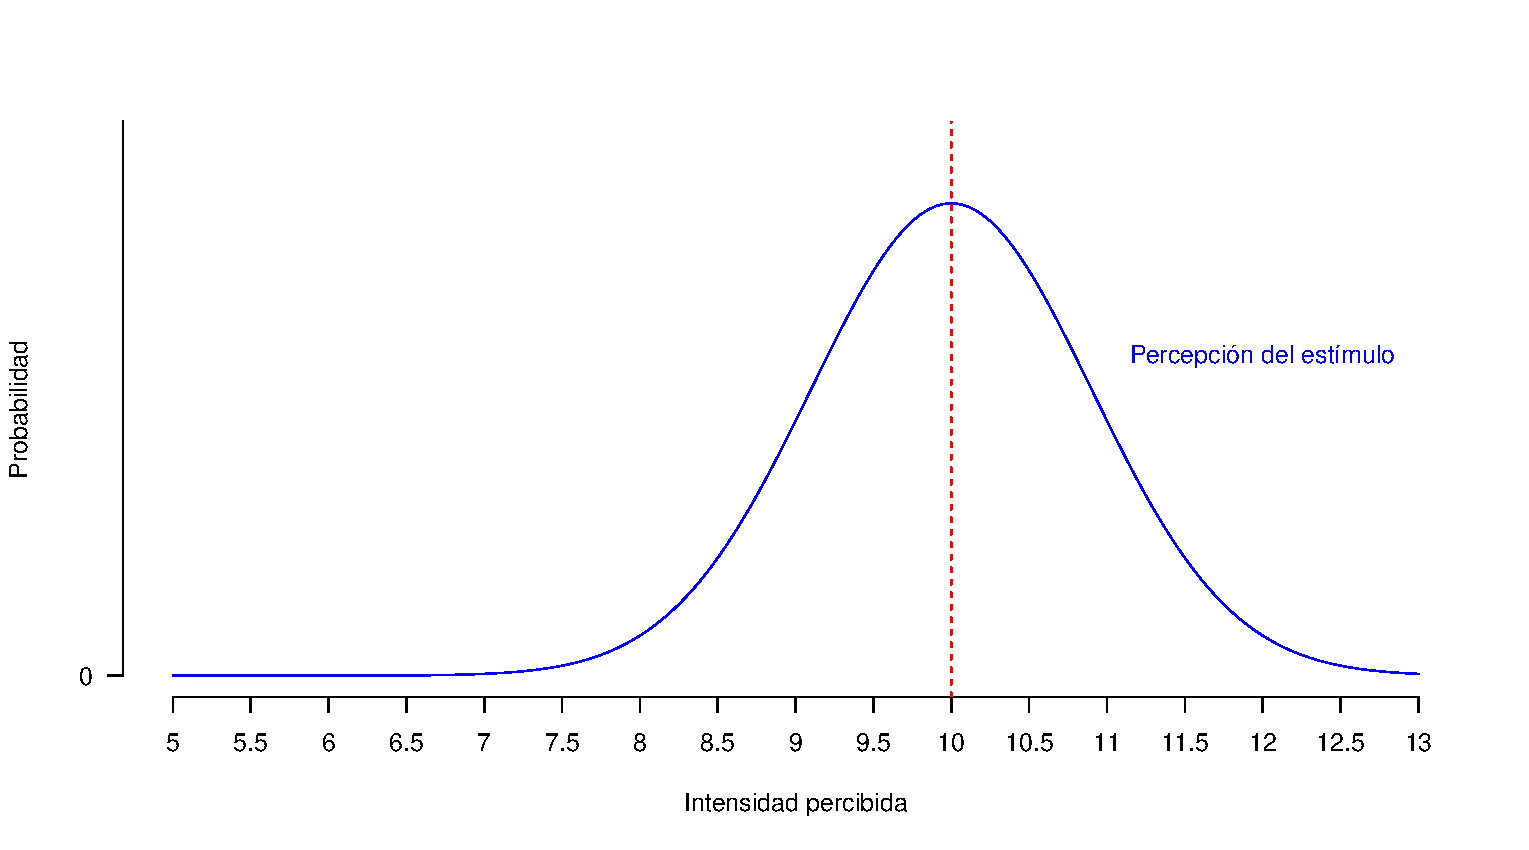
\includegraphics[width=0.70\textwidth]{Figures/Signal_Perception} 
%\decoRule
\caption[Variabilidad en la percepción de los estímulos]{Figura representativa de la variabilidad en la percepción de los estímulos. Si se presenta un mismo estímulo con intensidad x en repetidas ocasiones, es muy probable que el valor percibido se acerque a su valor real, (la media de la distribución, $\mu$) sin embargo y aunque con menor probabilidad, también habrán ocasiones en que sea percibido como más, o menos, intenso, (siendo cada vez menos probables conforme se alejan del valor 'real'.}
\label{fig:Senal_percepcion}
\end{figure}


\begin{figure}[th]
\centering
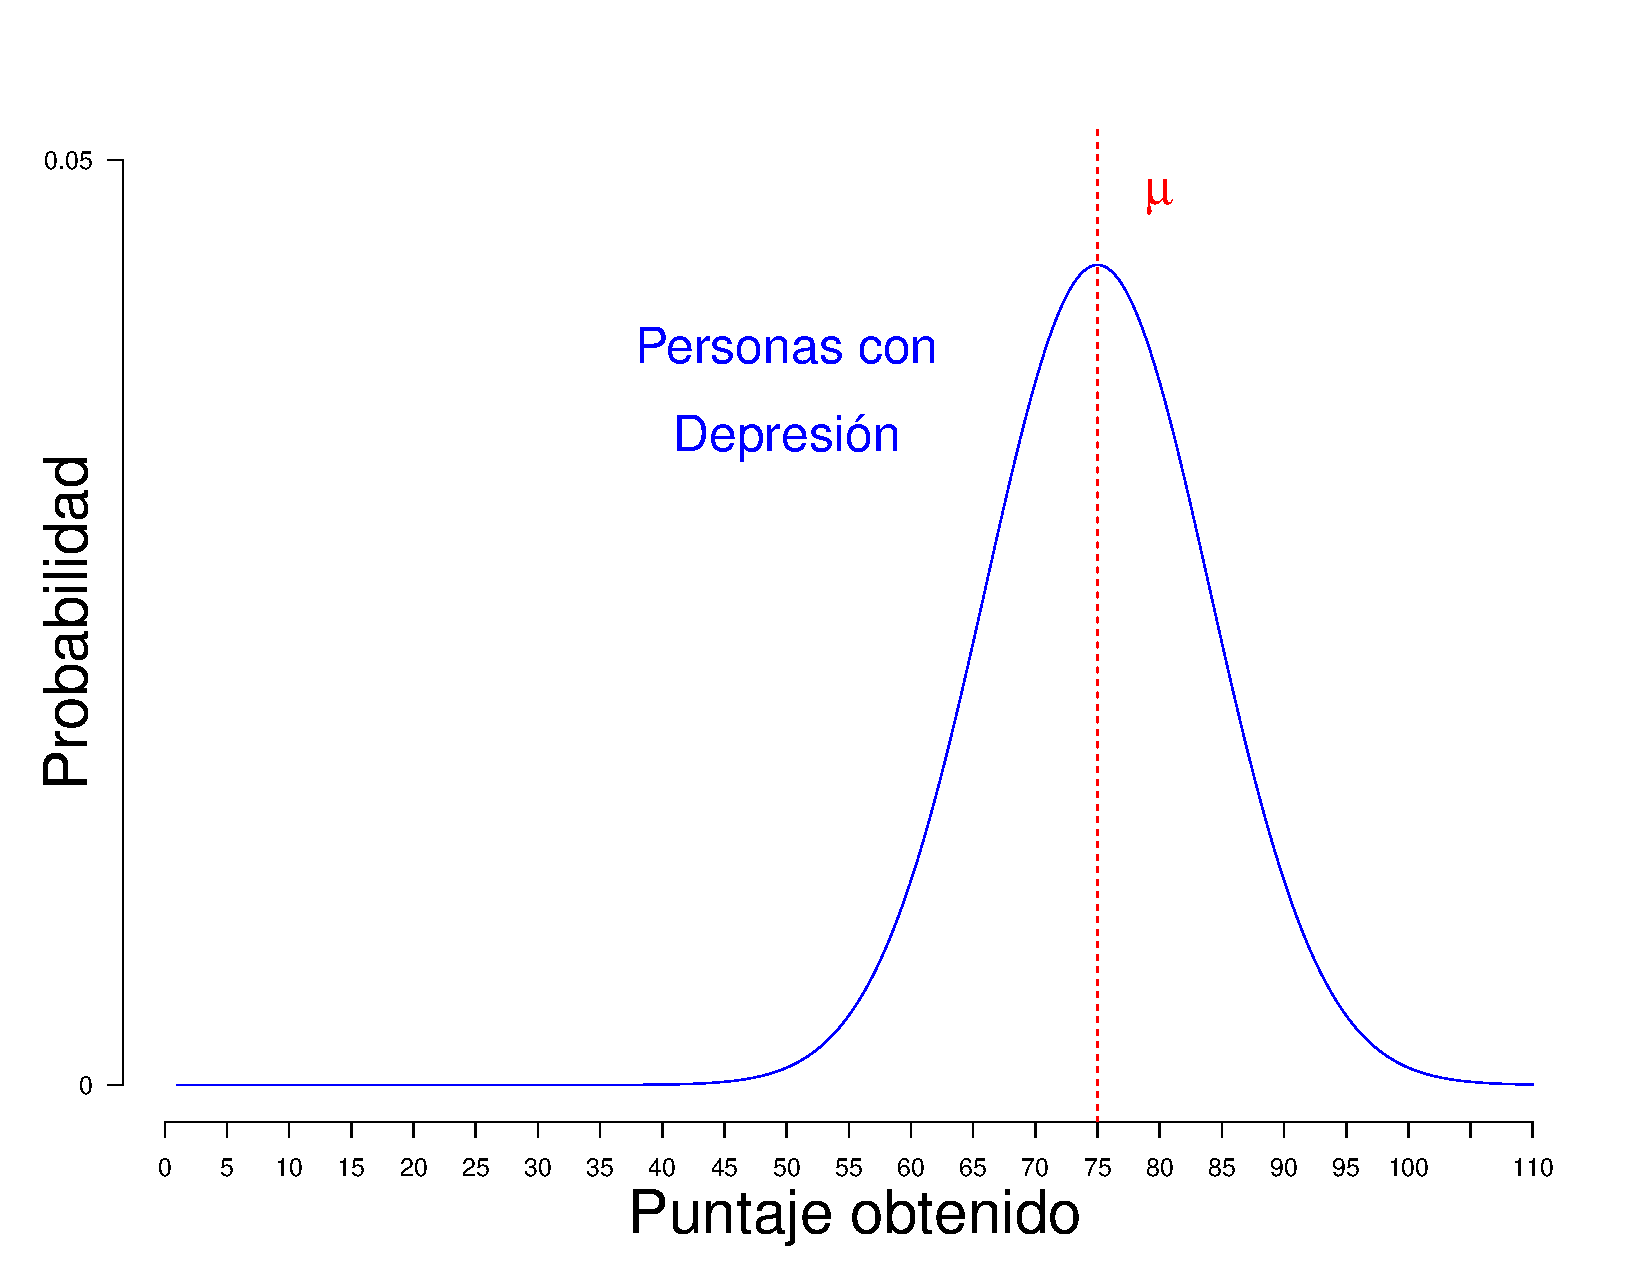
\includegraphics[width=0.70\textwidth]{Figures/Signal_Presentation} 
%\decoRule
\caption[Variabilidad en la presentación de los estímulos]{Figura representativa de la variabilidad en la presentación de los estímulos. Al aplicar una prueba clínica para detectar casos de Depresión, el diagnóstico emitido a partir de los puntajes observados se hace en relación a un rango identificado de valores que se asocian a dicha condición con mayor o menor probabilidad al rededor de una media ($\mu$, señalado en rojo). Los valores representados son arbitrarios.}
\label{fig:Senal_presentacion}
\end{figure}


En general, las Figuras~\ref{fig:Senal_percepcion} y \ref{fig:Senal_presentacion} representan un elemento fundamental para la forma en que la TDS concibe la detección de señales como un problema de adaptabilidad: la variabilidad es intrínseca a la presentación de los estímulos, ya sea porque nuestros sistemas sensoriales no los capturan igual en cada presentación, o porque los estímulos no se nos presentan exactamente de la misma forma en cada ocasión. Es decir, los estímulos en cuya detección están interesados los organismos (las señales) son variables en sí mismos, \parencite{Tanner1954}.\\

    \underline{b) La variabilidad en el Entorno: Ruido}\\

%La señal coexiste con el ruido y puede llegar a confundirse con el mismo.
Además del hecho de que existe variabilidad implícita en las señales a detectar, es necesario tomar en cuenta que estas coexisten en el mundo con otros estímulos o estados que -dada su propia variabilidad- pueden llegar a producir evidencia similar y confundir el diagnóstico de detección emitido por los organismos implicados en la tarea, \parencite{Tanner1954}.\\

Retomando el ejemplo planteado en la Figura~\ref{fig:Senal_presentacion} acerca de la variabilidad en los puntajes observados en personas con una condición particular en una prueba clínica, la Figura~\ref{fig:Noise} ilustra por añadidura un segundo punto clave para entender por qué se habla de la detección de señales como un problema con incertidumbre. Ya que así como las personas con depresión no obtienen siempre un mismo puntaje, no todas las personas que presentan la prueba sin tener la condición obtienen un cero absoluto -o cualquier otro puntaje fijo- como resultado, sino que a su vez obtienen puntajes dentro de su propia distribución de probabilidad (la distribución agregada en color negro). Nótese que existe un pequeño conjunto de valores a lo largo de los cuales se traslapan las dos distribuciones y tomemos en cuenta que las evaluaciones clínicas se realizan para detectar -diagnosticar- cierta condición en la persona evaluada -la señal- de acuerdo al resultado obtenido; ¿Cuál sería el diagnóstico pertinente para una persona que obtuvo 63 puntos en la prueba? Parece ser que dicha evidencia corresponde con lo observado tanto en los casos que contienen la señal, como en los que no. Sin embargo, dentro de este rango compartido de puntajes a observar en personas con o sin depresión, parece ser que existen algunos (los más cercanos a la media de la distribución de señal) que son más probables en personas con dicha condición, y viceversa. Sin embargo, el punto es claro: existe incertidumbre en la tarea en tanto que la señal y el ruido pueden llegar a producir la misma evidencia.\\ 

\begin{figure}[th]
\centering
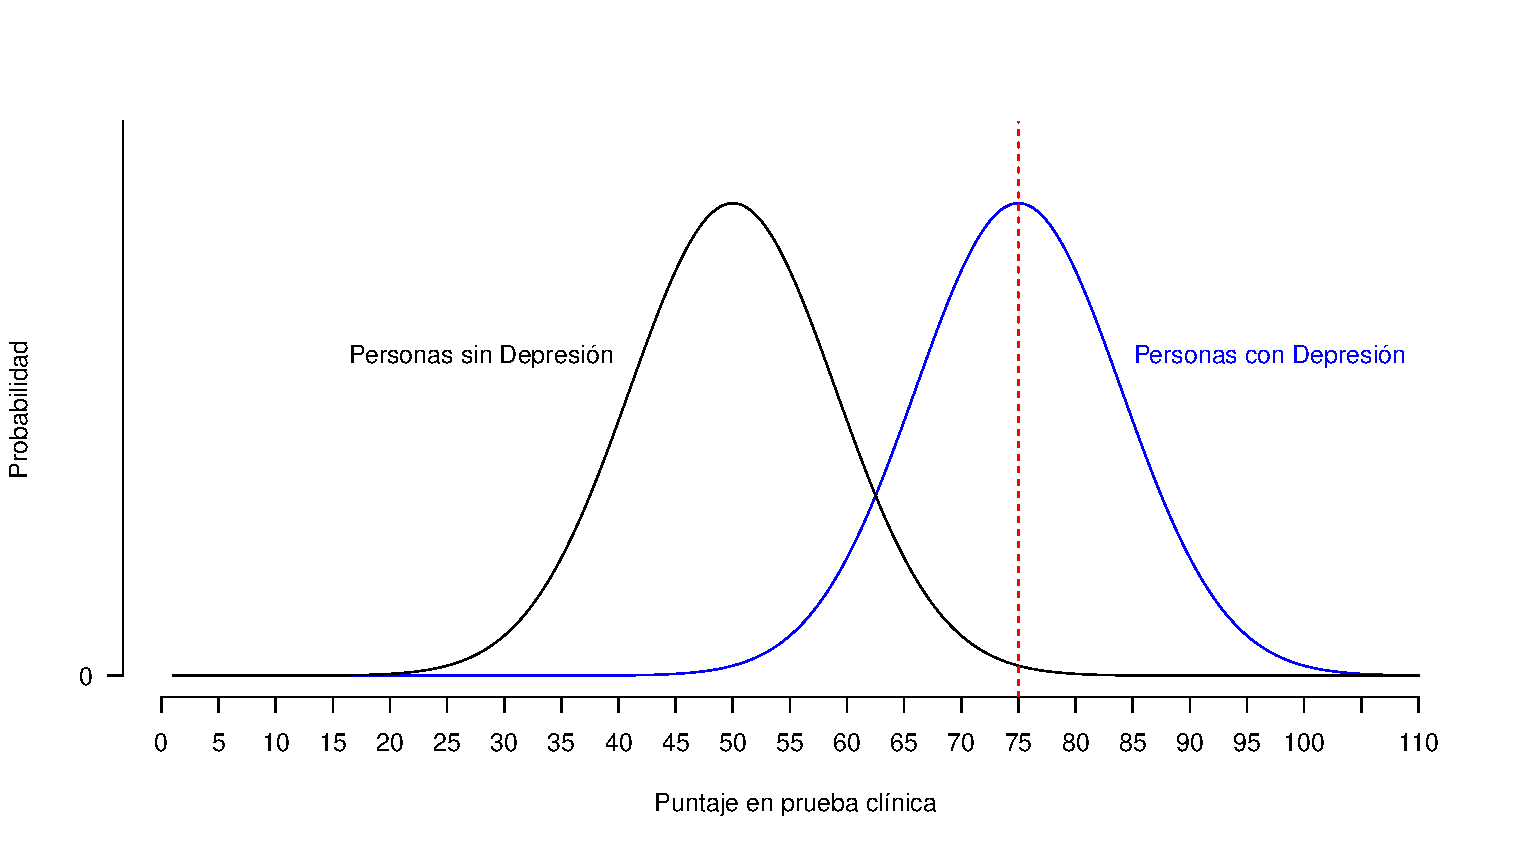
\includegraphics[width=0.70\textwidth]{Figures/Noise} 
%\decoRule
\caption[Variabilidad en la señal y en el ruido]{Extensión del ejemplo acerca de la aplicación de una prueba clínica para detectar casos de depresión. Se presenta una distribución para representa el rango de puntajes asociados con dicha condición (en azul) y se agrega una nueva distribución que representa el rango de puntajes observados en personas sin depresión que realizan esta misma prueba (en negro). La Figura ilustra la noción de que los posibles estados de mundo -señal y ruido- se presentan y perciben dentro de su propia variabilidad en cada ocasión, siendo posible que la evidencia producida se confunda entre sí. Los valores utilizados son arbitrarios.}
\label{fig:Noise}
\end{figure}

Al hablar de Discriminabilidad en tareas de detección bajo el marco de la TDS, se hace referencia a la probabilidad con que la señal y el ruido producen la misma evidencia (o bien, "¿qué tan probable es que la señal y el ruido se confundan?"). Y en términos de la representación gráfica del problema con sus respectivas distribuciones de probabilidad, implica una evaluación de qué tan grande es el área de sobrelape, al considerar esta un indicador fundamental de la incertidumbre contenida en la tarea ("¿Qué tan discriminable -diferente- es la señal respecto del ruido?").\\

La Figura~\ref{fig:Overlap} presenta dos figuras representativas que ilustran la relación entre la distancia entre las distribuciones de ruido y señal, el área de sobrelape entre estas y su interpretación en términos de la discriminabilidad de los estímulos contenidos en la tarea. En el panel superior (a), las distribuciones están muy separadas y el sobrelape entre estas es pequeño, sugiriendo un entorno con poca incertidumbre donde es muy poco probable encontrar evidencia que pueda confundir al organismo entre ambos estados del mundo -discriminabilidad alta-. Por otro lado, si las distribuciones están más juntas, como ocurre en el panel inferior (b), el sobrelape será cada vez mayor, indicando que existe un rango amplio de valores-evidencia vinculados simultáneamente con ambos estados del mundo y ante los cuales el organismo no podría tener certeza sobre a cuál de estos adjudicar su observación -discriminabilidad baja-.\\

\begin{figure}[th]
\centering
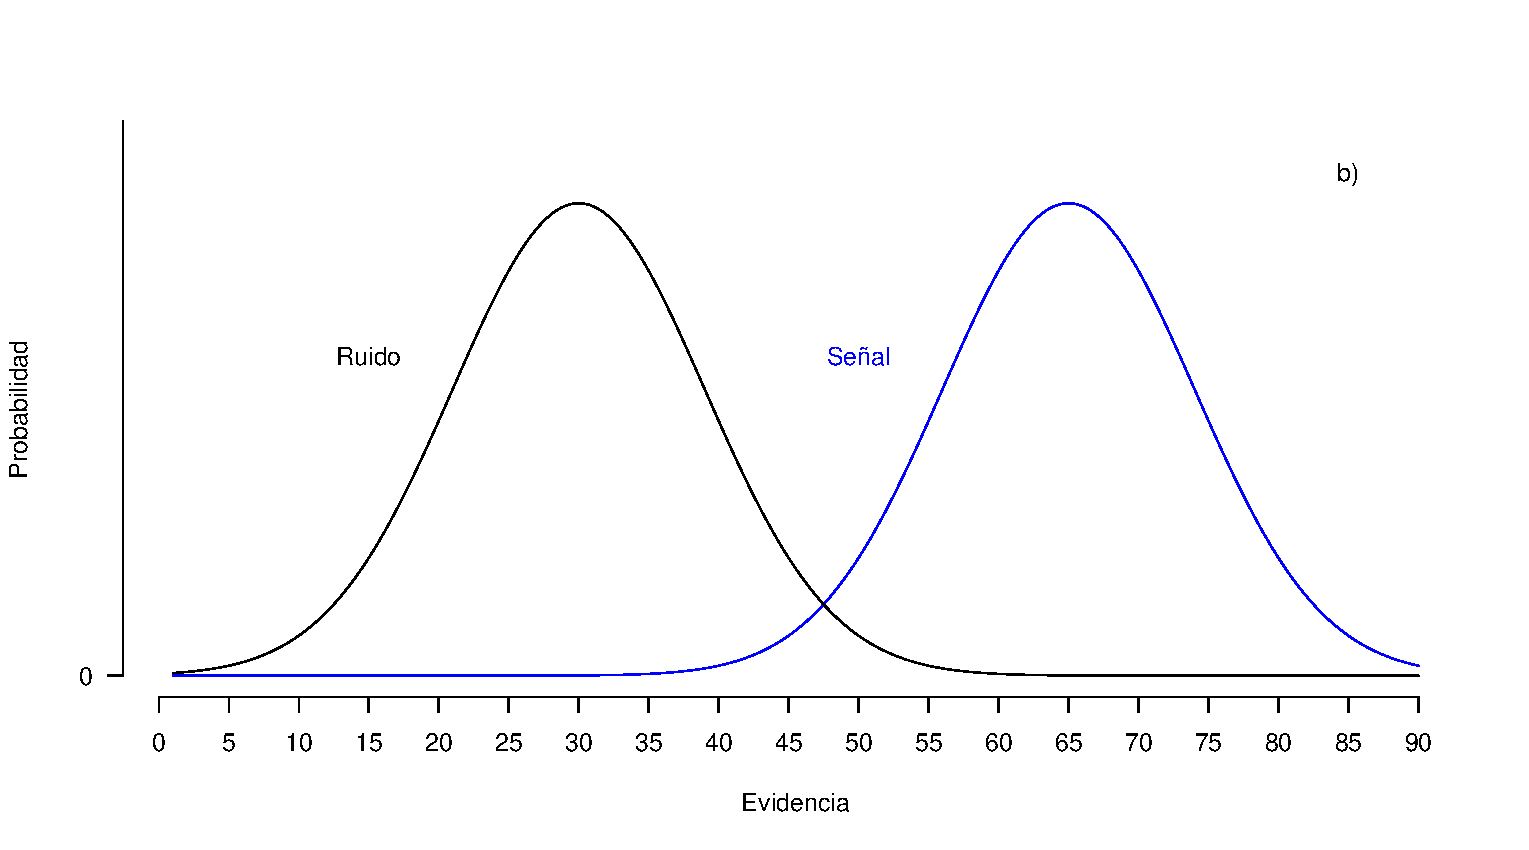
\includegraphics[width=0.55\textwidth]{Figures/Overlap_Small}\\ 
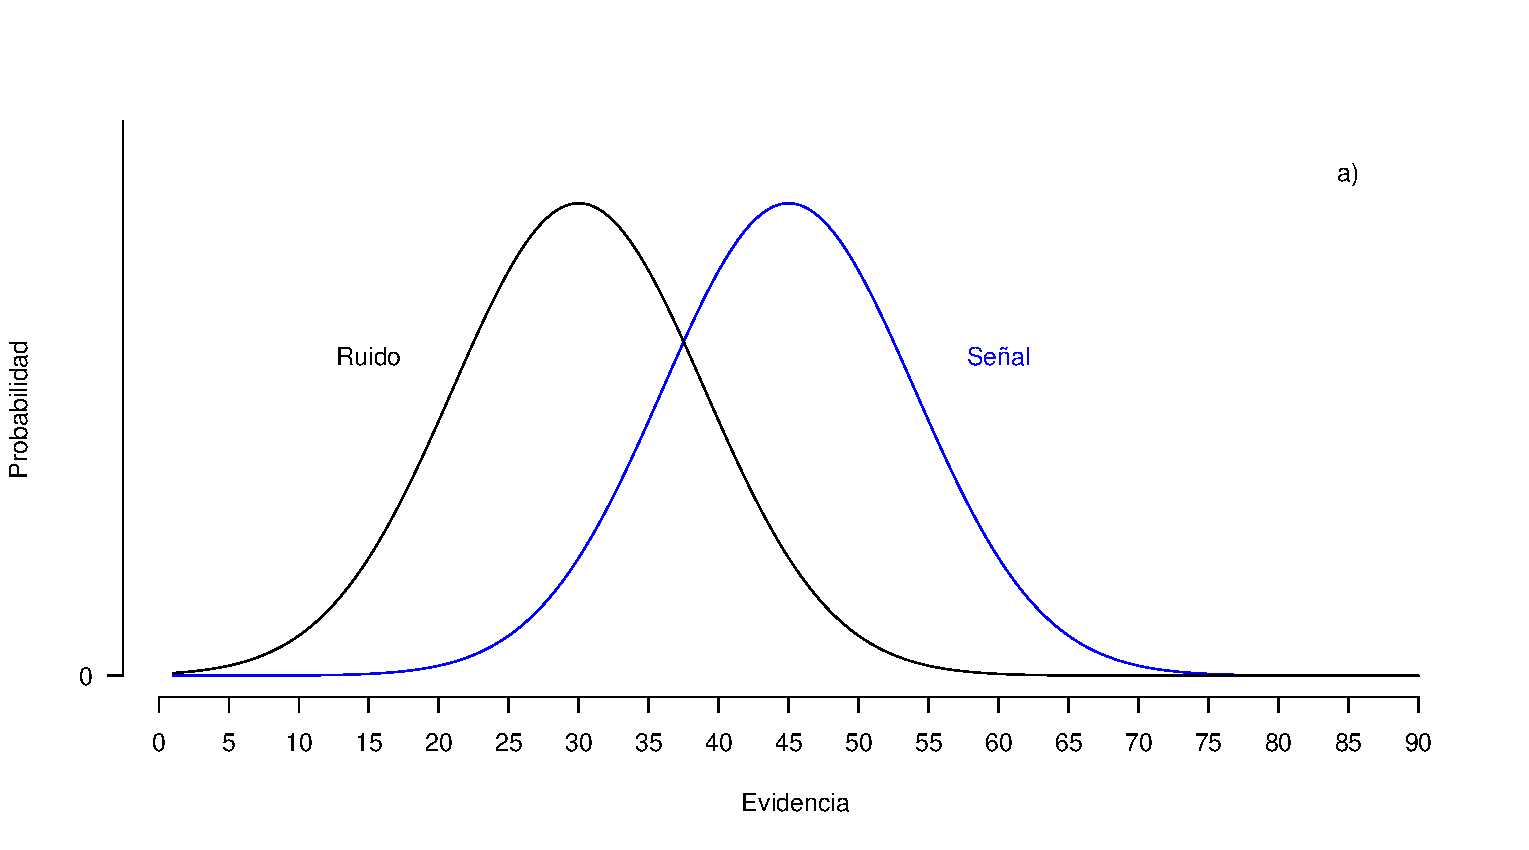
\includegraphics[width=0.55\textwidth]{Figures/Overlap_Big} 
%\decoRule
\caption[El sobrelape Ruido-señal como reflejo de la incertidumbre contenida en tareas de detección]{La distancia entre las distribuciones de ruido y señal determina la incertidumbre contenida en la tarea de detección al variar con ello el área de sobrelape entre las mismas. En el panel a) se presenta un ejemplo donde al estar muy separadas las distribuciones, el sobrelape es pequeño -poca incertidumbre-. En el panel b) se muestra un segundo escenario donde las distribuciones están más cerca, compartiendo más evidencia en el área de sobrelape -más incertidumbre-.}
\label{fig:Overlap}
\end{figure}

La Discriminabilidad en una tarea de detección es producto de la variabilidad con que los posibles estados del mundo se presentan y perciben por los sistemas detectores. Es decir, depende tanto de las propiedades intrínsecas de los estímulos a evaluar -¿qué tanto parecido tienen los estímulos con la señal y los estímulos sin esta?- como de la precisión con que los sistemas detectores son capaces de discernir entre dichas instancias -¿qué tan bueno es el organismo en distinguir una señal del ruido?-, \parencite{Nevin1969}. Por ejemplo, no es lo mismo tratar de detectar una manzana entre un montón de naranjas que entre un montón de melocotones y en general, esperaríamos que la tarea fuera más sencilla al tener una mayor discriminabilidad en el primer escenario; así mismo, la tarea de detectar cuando un instrumento musical no está afinado no es igual de difícil para un músico que para una persona sin educación musical.\\

  \textbf{2.- El papel del Sesgo: La detección es decisión}\\

La variabilidad en la presentación y percepción de los posibles estados del entorno -la presencia o ausencia de la señal- constituye el elemento base sobre el cual se desarrolla la TDS y que lleva a concebir la detección de señales como una tarea cargada de incertidumbre, donde los organismos no pueden confiar completamente en la evidencia que se les presenta para emitir un juicio de detección puesto que esta puede relacionarse con cualquiera de las interpretaciones posibles.\\

Los organismos compensan la incertidumbre contenida en las tareas de detección con la información que poseen sobre el entorno. En términos generales, esta puede ser de dos tipos: 1) información probabilística y 2) información sobre las consecuencias comprometidas, \parencite{Nevin1969}.\\

Imaginemos por ejemplo el caso de un médico que trata de decidir si los resultados obtenidos en cierta prueba clínica son evidencia suficiente para diagnosticar una enfermedad 'X' a un paciente 'Y'. La evidencia con la que el médico cuenta es imprecisa: toda prueba clínica tiene un margen de error y su lectura debe complementarse con información extraída de su historia clínica. El médico debe juzgar la evidencia en función de toda la información de la que dispone: ¿Qué tan confiable es la prueba?, ¿Cuál es su tasa de aciertos y errores?; ¿Qué tan común es la enfermedad cuya presencia se intenta determinar?, ¿Qué tan probable es que el paciente 'Y' tenga la enfermedad 'X'?; de acuerdo con su historia clínica, ¿qué tanto correlacionan sus características con los factores de riesgo asociados a la enfermedad?, ¿qué tanto cambia la probabilidad de que tenga la enfermedad 'X'?. Y la historia no termina aquí; la información probabilística permite hacer inferencias sobre cuál es la conclusión más probable, pero sigue sin haber certeza sobre el diagnóstico. Para optimizar su comportamiento y tomar la mejor decisión posible, el médico también debe tomar en consideración la información que posee sobre las consecuencias asociadas a cada escenario posible: a) Si el paciente tiene la enfermedad y el médico la detecta acertadamente, podrá tratarse a tiempo; b) Si tiene la enfermedad y el médico falla en detectarla, podría poner en riesgo su vida; c) Si no tiene la enfermedad y el médico le dice que sí, se gastarán recursos innecesarios en solucionar un problema que no existe, corriendo el riesgo de que el tratamiento le haga daño y d) Si no tiene la enfermedad y el médico decide no darle el diagnóstico, todo permanecerá igual. La tarea del médico es mucho más compleja de lo que parecía en un principio, puesto que no se limita a la lectura de una prueba clínica, sino a ponderar lo que sugieren los resultados de la misma con toda la información que posee sobre la probabilidad de las interpretaciones posibles y las consecuencias comprometidas.\\

De acuerdo con la correspondencia entre el estado real del mundo y el juicio emitido por el agente detector, se puede distinguir entre dos tipos de aciertos y errores. Tal y como se muestra en la matriz de contingencia presentada en la Figura~\ref{fig:Mat_Output}, en el marco de la TDS se habla de cuatro posibles resultados: cuando la señal está presente el organismo puede detectarla adecuadamente (Hit) o dejarla pasar (Omisión); a su vez, si la señal no está presente, el organismo puede acertar al diagnosticar su ausencia (Rechazo correcto) o confundir el ruido con la señal, (Falsa Alarma).\\

\begin{figure}[th]
\centering
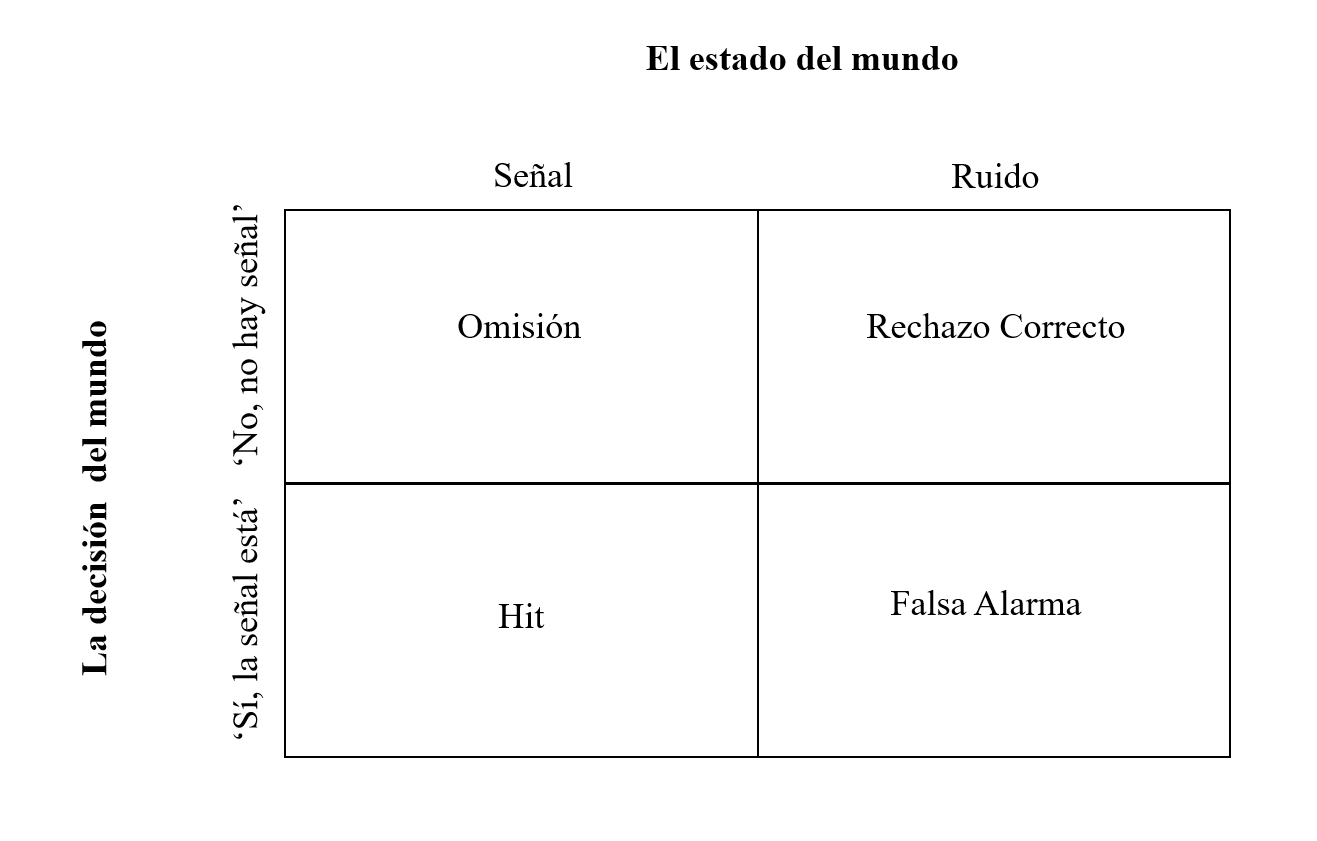
\includegraphics[width=0.60\textwidth]{Figures/Matriz_Outputs} 
%\decoRule
\caption[Posibles Resultados en una Tarea de Detección]{Los cuatro posibles resultados que se espera encontrar de acuerdo con la TDS, dada la incertidumbre contenida en las tareas de detección, en función de la correspondencia que existe entre los juicios emitidos por los organismos y el estado real del mundo.}
\label{fig:Mat_Output}
\end{figure}

La TDS asume que con base en la información de la que dispone sobre la estructura de la tarea, el organismo fija un criterio de elección para determinar a partir de cuánta evidencia va a juzgar la presencia de la señal dado lo que sabe sobre la probabilidad con que ésta ocurre y las consecuencias comprometidas con su detección, \parencite{Tanner1954, Swets1961, Nevin1969}. En términos de la representación gráfica del modelo, implica que sobre el eje de la Evidencia el organismo sitúa una línea vertical que atraviesa ambas distribuciones y que va a fungir como regla de elección para delimitar a partir de cuánta evidencia  emitir juicios de detección en favor de la señal,como se ilustra en la Figura~\ref{fig:Graf_Outputs} con una línea roja.\\

\begin{figure}[th]
\centering
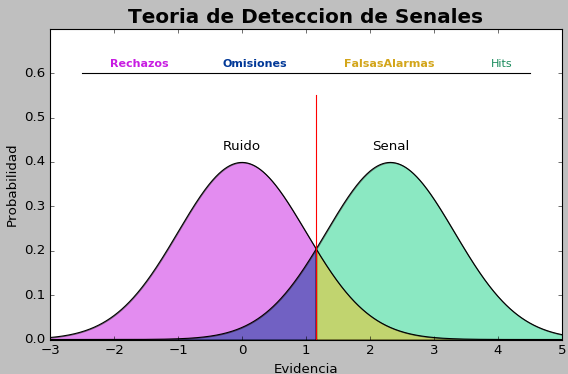
\includegraphics[width=0.60\textwidth]{Figures/Graficador_Tasas} 
%\decoRule
\caption[Posibles Resultados en una Tarea de Detección]{Representación gráfica del problema de detección de señales de acuerdo con la TDS. Existe una distribución de probabilidad que describe las formas en que la señal se presenta en el entorno y una distribución que corresponde a los demás estímulos. Como resultado del traslape entre estas -incertidumbre- el organismo fija un criterio de elección (la línea roja) para determinar a partir de cuánta evidencia juzgará la presencia de la señal, y que determina la probabilidad de obtener cualquiera de los resultados señalados en la figura con distintos colores.}
\label{fig:Graf_Outputs}
\end{figure}

La Figura~\ref{fig:Graf_Outputs} presenta -de forma mucho más completa que las figuras antes mostradas en este capítulo- la forma en que se representan los problemas de detección de señales bajo el marco de la TDS: Se tienen distribuciones de probabilidad que representan la variabilidad con que la señal y el ruido ocurren en el ambiente, \parencite{Tanner1954} y una línea roja que señala el criterio que va a utilizar el agente detector para emitir un juicio de detección. La localización del criterio de elección determina la probabilidad con que, de acuerdo a la cercanía de las distribuciones (discriminabilidad), se esperaría incurrir en cada uno de los cuatro resultados expuestos en la matriz de contingencia de la figura~\ref{fig:Mat_Output}.\\

Dada la estructura de la tarea y el conocimiento que el organismo tenga sobre ella, es posible que se desarrolle una tendencia que favorezca la emisión de un juicio de detección particular, \parencite{Nevin1969}. Esto es lo que en el marco de la TDS se identifica como Sesgo. Se asume que la localización del criterio sobre el eje de evidencia es un reflejo del mismo y que su magnitud y dirección depende de dos grandes factores:\\


      \underline{a) Los errores cuestan y los aciertos pagan: Matrices de pago}\\

La variabilidad contenida en la presentación de los estímulos presentes en situaciones de detección da la pauta para que los sistemas inmersos en ellas corran el riesgo de cometer errores.\\

Para entender la importancia en términos de la adaptabilidad de los organismos de las situaciones de detección, es importante recordar que la detección de señales funge como un filtro para orientar su conducta en términos de las consecuencias involucradas. En otras palabras, acertar en un juicio de detección trae consigo ciertas ventajas -derivadas de la adecuada identificación de las reglas operantes en el entorno- y errar cuesta. Y más aún, los distintos tipos de aciertos y errores comprometidos, pagan y castigan en distinta medida.\\

Imaginemos el caso de un animal indefenso -un conejo- que tiene que decidir tan rápido como pueda si el sonido que acaba de escuchar en la maleza corresponde, o no, con el de un depredador. La penalización asociada con cometer una falsa alarma -un gasto innecesario de energía al correr para nada- es sustancialmente diferente a el precio que tendría que pagar por incurrir en una omisión -¡la muerte!-. Dadas las consecuencias en juego, es muy probable que el conejo decida actuar en consecuencia de un juicio de detección afirmativo ("¡Sí, es un depredador!") y correr por su vida, aún ante niveles de evidencia muy bajos.\\

\begin{figure}[th]
\centering
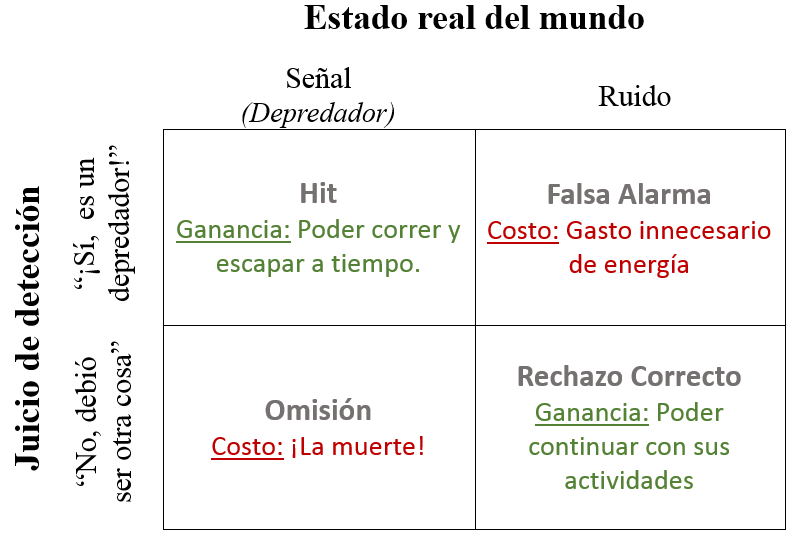
\includegraphics[width=0.60\textwidth]{Figures/Matriz_Pagos} 
%\decoRule
\caption[Ejemplo de Matriz de Pagos]{De acuerdo con el ejemplo planteado en el capítulo acerca de la tarea de detección a la que se enfrenta un conejo que intenta determinar si los sonidos que escucha en su entorno corresponden con los de un depredador, se presenta una matriz de pagos que ilustra los costos y ganancias comprometidos en la tarea en función a la correspondencia entre el juicio elegido y el estado verdadero del mundo.}
\label{fig:Mat_Pagos}
\end{figure}

La figura~\ref{Mat_Pagos} presenta lo que en los modelos clásicos de decisión se conoce como una Matriz de Pagos y que se utiliza para señalar, de acuerdo a una matriz de contingencia, los costos y ganancias asociados con cada resultado observable en tareas de detección. En términos de la TDS, se asume que los organismos toman en cuenta esta información para definir la localización de su criterio de elección. En otras palabras, ya que los organismos nunca podrán tener certeza absoluta sobre los juicios de detección emitidos, se juzga la evidencia a partir de un criterio de elección que toma en cuenta las consecuencias comprometidas en un intento por optimizar su conducta y los resultados obtenidos, \parencite{Killeen2014}.\\

      \underline{b) Estimados de Probabilidad}\\

Los organismos involucrados en cualquier tarea de detección tienen alguna expectativa respecto de la probabilidad con que las señales de interés ocurren en el mundo. Es decir, ya sea como resultado de su experiencia directa o porque es información que les ha sido proporcionada de manera externa, \parencite{Nevin1969} los agentes detectores evalúan la evidencia con base en dos grandes probabilidades: 

\begin{itemize}
\item \textsl{Un estimado prior.} Con independencia de cuál sea la evidencia evaluada de manera inmediata, ¿qué tan probable es encontrar la señal en esta situación particular?\\

Si los organismos se encuentran en un entorno donde saben que es prácticamente imposible encontrar la señal, es muy probable que decidan descartar la evidencia que se les presente aún si esta correlaciona con lo que se esperaría de una señal. Por ejemplo, recordemos el ejemplo planteado con anterioridad sobre querer determinar la edad de una persona al hablar con ella por teléfono: si la llamada fue hecha a un despacho de abogados -o cualquier otro escenario donde se piense que es muy poco probable encontrar a un niño-, aún si la persona al otro lado del teléfono tiene una voz muy aguda, es muy poco probable que su interlocutor piense "Oh, estoy hablando con un niño".\\

\item \textsl{La verosimilitud.} Dado lo que se sabe sobre cómo se presentan ciertos estímulos en el entorno -incluyendo la señal-, ¿qué tan verosímil es la evidencia? o bien, ¿qué tan probable exactamente es que la señal o el ruido se presenten con la evidencia que se está evaluando de manera inmediata?\\

Asumir que los organismos apoyan su juicio de detección en el conocimiento que tienen sobre la verosimilitud de la evidencia, es el equivalente a suponer que tienen alguna idea sobre cómo se ven las distribuciones de probabilidad que rigen la ocurrencia del ruido y señal. Bajo este escenario, ante la incertidumbre -si los organismos se enfrentaran a evidencia que cae en el área de sobrelape entre las distribuciones- los agentes detectores optarían por elegir el juicio de detección que corresponda con la distribución que se asocie con dicha evidencia con mayor probabilidad (es decir, la distribución que sea más alta en ese punto particular del eje de decisión), \parencite{Nevin1969}.\\
\end{itemize}

De contar con ambos elementos, es posible asumir que los organismos se decantan por un juicio de detección particular con base en el conocimiento que tienen sobre la estructura probabilística del entorno, mediante la realización de una inferencia bayesiana \parencite{WeijiMa, WeijiMa2012, Pouget2013}.\\

\subsection{Parámetros del modelo}\\

La TDS, además de proporcionar un modelo estadístico para comprender las implicaciones adaptativas del problema de la detección, funge como una herramienta que -dados los supuestos que hace sobre este tipo de tareas- permite hacer estimaciones sobre la discriminabilidad y el sesgo del sistemas inmersos en tareas de detección particulares, \parencite{Stainslaw1999, McNicol1}.\\

Las tareas de detección diseñadas en el laboratorio para estudiar el desempeño de los participantes experimentales sometidos a ellas, suelen estar compuestas por un amplio número de ensayos, a lo largo de los cuales se presentan la señal y ensayos con sólo ruido. Dependiendo lo que quiere evaluarse con la tarea, pueden implementarse manipulaciones adicionales, \parencite{Nevin1969}. Los protocolos que guían la presentacipon de tareas de detección se presentan con mayor detalle más adelante (Sección 2.1.3).\\

Al someter un sistema detector a una misma tarea de detección con incertidumbre en repetidas ocasiones (como ocurre en tareas experimentales), se espera encontrar variabilidad en las respuestas y resultados observados; el agente detector no acertará o errará consistentemente. Con base en las respuestas reportadas por los participantes en cada ensayo y el resultado obtenido en función a su correspondencia con el tipo de estímulo presentado, se computan las tasas con que se observaron cada uno de los posibles aciertos y errores. Es decir, dentro del total de veces que se presentó la señal, se identifica cuántas veces se cometió un Hit o una Omisión; y dentro del total de veces que se presetó sólo Ruido, la proporción de ensayos en que el participante hizo un Rechazo correcto o una Falsa alarma.\\

De acuerdo a la forma clásica de la TDS, las tasas de ejecución registradas en tareas de detección de señales son un reflejo del área de las distribuciones de Ruido y Señal que caen a ambos lados del criterio y pueden utilizarse para hacer inferencias sobre la localización del mismo, la distancia entre las distribuciones involucradas y la preferencia que podría tener el sistema por emitir una respuesta sobre otra, \parencite{Wickens, McNicol1, Gescheider, Stainslaw1999}. Acontinuación, revisaremos en detalle cuáles son los parámetros incluidos en el modelo de detección de señales, cómo se calculan y qué información arrojan sobre la ejecución de los participantes.\\

  \textbf{Supuestos formales}\\

La estimación paramétrica del modelo de detección de señales se desarrolla en torno a una serie de supuestos formales -pequeñas especificaciones técnicas- que facilitan la interpretación de los datos obtenidos a la luz de la representación gráfica propuesta por la TDS, \parencite{Wickens, Gescheider, Stainslaw1999}.\\ 

\begin{enumerate}

\item  Dado que las cuatro tasas de ejecución de los participantes se computan en función a dos conjuntos totales -total de estímulos con Señal y Ruido-, sólo se necesita computar un par de ellas. Por consenso general, en la literatura suelen usarse sólo las tasas de Hits y Falsas Alarmas -los aciertos y errores obtenidos cuando el participante respondió "Sí, detecto la señal"- para guiar las estimaciones a realizar sobre la tarea; las tasas de Omisiones y Rechazos correctos no proporcionan información adicional, en tanto que son el complemento de las primeras dos, respectivamente.\\

\item En su forma clásica, la TDS asume que las distribuciones de ruido y señal son distribuciones normales equivariantes, \parencite{Stainslaw1999}.\\
  \begin{itemize}
  \item Se utilizan distribuciones Gaussianas como el 'default' para describir la variabilidad contenida en cualquier conjunto de estímulos con señal y ruido, a falta de información específica y detallada sobre estos. Sin embargo, existe literatura que explora la conveniencia de representar la incertidumbre con otro tipo de distribuciones, \parencite{Wickens, WeijiMa2009}.\\
  \item En la mayoría de sus aplicaciones, se asume que las distribuciones de ruido y señal comparten una varianza de 1, \parencite{Tanner1954}. No obstante, específicamente hablando en términos de la aplicación del modelo al área de la Memoria de Reconocimiento, este supuesto es desechado en tanto que se ha encontrado evidencia consistente que sugiere que la distribución de señal (la distribución de estímulos ya antes presentados a reconocer) tiene una varianza mayor que la del ruido, \parencite{Wixted2007}. Las implicaciones de este hallazgo se discuten a profundidad más adelante.\\
  \end{itemize}
\item Se asigna de manera arbitraria una media en 0 a la distribución de ruido, para facilitar el cómputo del resto de los parámetros. En otras palabras, la media de la distribución de ruido funge como punto de referencia para la estimación paramétrica, \parencite{Wickens, Gescheider}.\\
\item Sin tratarse explícitamente de un supuesto formal hecho por la teoría, una de las implicaciones directas de la forma en que está constituida es que, sea cual sea la evidencia con base en la cual se asume que los organismos están formando los juicios de detección -los valores en el eje X sobre los cuales se despliegan las distribuciones-, se espera que la Señal tenga 'más' que el Ruido (en tanto que este último implica su ausencia), \parencite{Stainslaw1999}.\\
  \begin{itemize}
  \item La tasa de Falsas Alarmas no puede ser más grande que la tasa de Hits, puesto que esto implicaría que hay una mayor área de la distribución de ruido rebasando el criterio que de la distribución de la señal. De acuerdo con la representación del modelo, esto sugeriría que el ruido cae por encima de la señal en términos de la evidencia que produce y estaría violando el supuesto fundamental de que la señal -la presencia de lo que queremos detectar- contiene más información que el ruido -su ausencia-.\\
  \end{itemize}
\end{enumerate}

Los parámetros contemplados por el modelo evalúan el desempeño de los participantes en términos de los dos grandes factores que se asocian con la emisión de juicios de detección: la discriminabilidad y el sesgo. La aplicación exitosa de la TDS al estudio de una amplia gama de tareas de detección -que pueden variar desde el tipo de estímulos utilizados hasta el dominio o fenomeno a estudiar- es posible gracias a la abstracción de sus elementos. Los valores y el tipo de evidencia específicos sobre los cuales se despliegan las distribuciones de Ruido y Señal no importan tanto -de hecho, no suelen tomarse en cuenta- como saber qué tanto sobrelape había entre las distribuciones y qué juicio de detección era emitido con preferencia.\\

\begin{itemize}
\item \underline{Criterio ($k$)}\\

La localización del criterio sobre el eje de decisión se puede computar de manera directa, tomando como referencia el valor asignado -de manera arbitraria- por el modelo de la TDS a la media de la distribución de ruido (0), con base en las tasas de ejecución observadas en nuestro participante. \\

\begin{figure}[th]
\centering
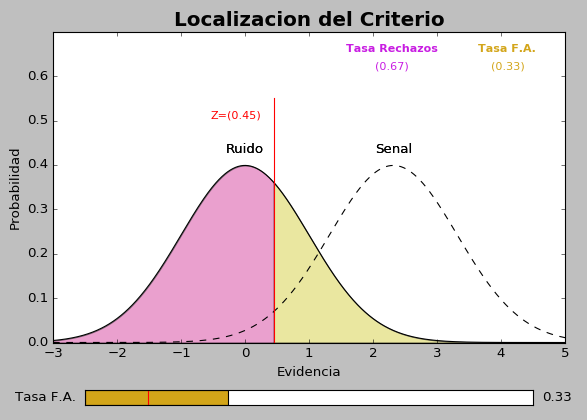
\includegraphics[width=0.60\textwidth]{Figures/Graficador_Criterio} 
%\decoRule
\caption[Estimación del criterio con base en las Falsas Alarmas]{La imagen presenta una captura de pantalla de un Graficador desarrollado por parte la autora de la presente tesis, como parte de un proyecto PAPIME trabajado en el Laboratorio 25, \parencite{PAPIME}}
\label{fig:Graf_Criterio}
\end{figure}

El parámetro $k$ representa la localización del criterio sobre el eje de decisión en unidades de Desviación Estándar, \parencite{Tanner1954}. Su cómputo implica interpretar la tasa de Falsas Alarmas como reflejo de la probabilidad acumulada -el área bajo la curva- de la distribución de Ruido que cae por encima del criterio y la tasa de Rechazos Correctos, como su complemento. Dado que -de acuerdo con los supuestos formales previamente expuestos- se asume que la distribucion de Ruido tiene media en 0 y desviación estándar de 1, la tasa de Rechazos Correctos puede transformarse en Puntajes Z para obtener un estimado -tomando como unidad la Desviación Estándar- de dónde se sitúa el criterio de elección, tomando como referencia la media de la distribución de Ruido. La Figura~\ref{fig:Graf_Criterio} ilustra este proceso, presentando como ejemplo una tasa de Falsas Alarmas arbitraria y la tasa de Rechazos Correctos complementaria, que al ser transformada a puntajes Z permite evaluar la localización del criterio respecto del 0 de referencia planteado por la distribución de ruido. Es decir:\\

\begin{center}
$k = PuntajeZ(Tasa de Rechazos Correctos)$\\
\end{center}

De acuerdo con los supuestos hechos por el modelo, el parámetro $k$ se expresa como un número real que señala -en unidades de Desviación Estándar (Puntajes Z)- la posición del criterio en relacióna la media de la distribución de Ruido.\\

\item \underline{Discriminabilidad ($d'$)}\\

La discriminabilidad se evalúa con un parámetro ($d'$) que define la distancia entre las medias de las distribuciones de Ruido y Señal, \parencite{Tanner1954}. Dado que a la distribución de Ruido le ha sido asignada una media en 0, también podemos pensar en $d'$ como reflejo de la localización de la media de la distribución de Señal.\\ 

Una vez determinada la localización del criterio relativa a la media de la distribución de Ruido con base en las tasas de Falsas Alarmas y Rechazos Correctos observadas, es sencillo concebir el cómputo de $d'$ como una extensión de dicho proceso; utilizando adicionalmente las tasas de Hits y Omisiones para conocer la localización de la distribución de Señal sobre el eje de evidencia, de manera que la probabilidad acumulada (el área bajo la curva) que cae por encima y por debajo del criterio coincidan con estas.\\ 

\begin{figure}[th]
\centering
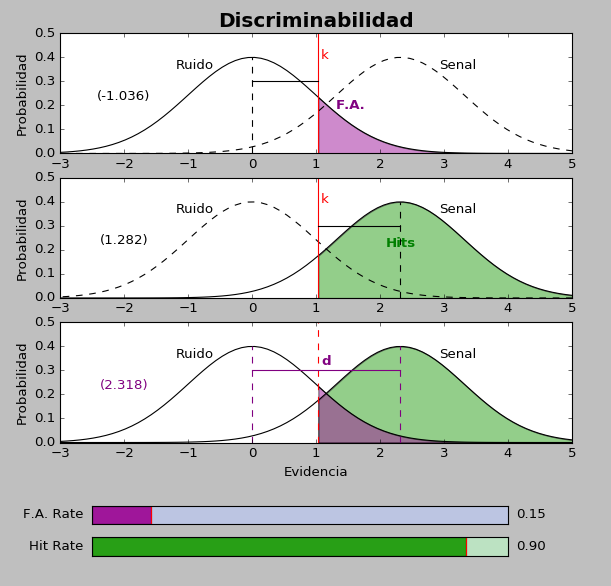
\includegraphics[width=0.75\textwidth]{Figures/Graficador_Discriminabilidad} 
%\decoRule
\caption[Estimación de la discriminabilidad con base en las Tasas de Ejecución]{La imagen presenta una captura de pantalla de un Graficador desarrollado por parte la autora de la presente tesis, como parte de un proyecto PAPIME trabajado en el Laboratorio 25, \parencite{PAPIME}}
\label{fig:Graf_Discrim}
\end{figure}

La Figura~\ref{fig:Graf_Discrim} ilustra la secuencia lógica de pasos que guían el cómputo del valor de $d'$:\\

\begin{enumerate}
\item En el panel superior, la tasa de Falsas Alarmas (señalada en color púrpura) es convertida a Puntajes Z.\\

Pese a que conceptualmente interpretamos la tasa de Falsas Alarmas como la probabilidad acumulada a la derecha del criterio (y esperaríamos tuviera un valor de Puntaje Z positivo), el valor obtenido es negativo porque la conversión de un cierto valor de probabilidad acumulada a Puntajes Z sólo puede hacerse bajo el entendido de que dicha probabilidad es acumulada de izquierda a derecha (y no al revés, como implica nuestra interpretación). Es decir, que el Puntaje Z obtenido para la tasa de Falsas Alarmas es negativo porque, al ser menor a 0.5, se le asigna un Puntaje Z como si la distribución hubiese sido invertida y la probabilidad acumulada representada se situara a la izquierda, por debajo de la media.\\

El primer panel representa la distancia entre el criterio y la media de la distribución de Ruido.\\

\item El panel intermedio muestra el resultado de transformar la tasa de Hits (señalada en color verde) en puntajes Z.\\

A pesar de que el criterio golpea la distribución de Señal por debajo de la media (la probabilidad acumulada señalada por la tasa de Hits se aglomera de derecha a izquierda), el puntaje Z obtenido es positivo porque -nuevamente- la tasa de Hits es interpretada como una probabilidad acumulada de izquierda a derecha. Dado que la tasa de Hits suele ser mayor al azar ($TasadeHits > 0.5$), el puntaje Z resultante es positivo porque, leyéndose de izquierda a derecha, representa un área bajo la curva que caería por encima de la media de la distribución de Señal.\\

El segundo panel muestra la distancia entre el criterio y la media de la distribución de Señal.\\

\item El panel inferior presenta la idea detrás del cómputo de $d'$: la suma de las distancias entre el criterio y las medias de cada una de las distribuciones. En otras palabras:\\

\begin{center}
$d' = PuntajeZ(Tasa de Hits) - PuntajeZ(Tasa de Falsas Alarmas)$\\
\end{center}

\end{enumerate}

El parámetro $d’$ sólo puede tener valores positivos ya que la teoría asume que la distribución de Señal siempre se sitúa a la derecha de la distribución de Ruido porque contiene una mayor cantidad de la evidencia con base en la cual se hace el juicio de detección de la señal, \parencite{Stainslaw1999}. El valor de $d'$ es un reflejo de la discriminabilidad en la tarea (la distancia entre las distribuciones); si $d' = 0$, querría decir que las distribuciones de Ruido y Señal están completamente sobrelapadas y es imposible distinguir entre ellas ("No hay discriminabilidad entre los estímulos"). \\

\item \underline{Sesgo ($\beta$ y $C$)}\\

La TDS cuenta con dos parámetros que permiten evaluar la magnitud y la dirección del sesgo bajo el cual se está respondiendo a la tarea, \parencite{Stainslaw1999, Macmillan1996}.\\

\begin{itemize}
\item \underline{$\beta$}\\

El parámetro más comúnmente reportado en la literatura es Beta ($\beta$), que se define como la razón entre la probabilidad con que la evidencia que se presenta a la altura del criterio corresponde con la distribución de Señal y la probabilidad con que podría representar una instancia del Ruido: \\

\begin{center}
$\beta = \frac{p(Signal)}{p(Noise)}$ \\
\end{center}

\item \underline{$C$}\\

Un segundo parámetro para computar el sesgo es $C$, que representa la distancia entre la localización del criterio utilizado por el participante sometido a la tarea y el punto de intersección entre las distribuciones ($\frac{d'}{2}$):\\

\begin{center}
$C =  K - \frac{d'}{2}$ \\
\end{center}

Se utiliza $\frac{d'}{2}$ como punto de referencia para evaluar el sesgo del sistema porque se asume que esta debería ser la localización del criterio a utilizar por un sistema sin sesgo, ya que el área de las distribuciones que caería por encima y por debajo de este punto son idénticas y parecieran reflejarse entre sí. En otras palabras, un criterio en $\frac{d'}{2}$ implicaría la misma probabilidad de cometer ambos tipos de aciertos y errores. Por ello, el sesgo del sistema detector observado se evalúa a partir de su comparación directa con este punto neutro.\\

\end{itemize}

El sesgo puede ser evaluado en términos de dos grandes factores: 1) ¿Qué tan sesgado está el sistema? y 2) ¿Cuál es el juicio de detección que se está favoreciendo?\\

El parámetro $\beta$ indica cuántas veces es más probable que la evidencia observada a la altura del criterio corresponda con la Señal. Valores de $\beta$ por encima de 1, sugieren que el punto en que la distribución de Señal toca el criterio es más alto que en la distribución de Ruido; es decir, el sistema detector no emite juicios afirmativos hasta que exista una alta probabilidad de correspondencia entre la evidencia evaluada y la variabilidad contenida en la Señal y, por el contrario, emite juicios negativos con mayor probabilidad. Valores de $\beta$ entre 0 y 1, por su parte, sugieren que es más probable que la evidencia encontrada a la altura del criterio provengan de la distribución de Ruido que de la de Señal; esto indicaría que el sistema detector está emitiendo juicios afirmativos aún cuando es más probable que la evidencia observada corresponda con el Ruido. Cuando el criterio del participante coincide con el criterio neutro previamente descrito ($\frac{d'}{2}$), $\beta$ vale exactamente 1, pues tocaría ambas distribuciones a la misma altura.\\

El valor absoluto del parámetro $C$ proporciona información sobre la magnitud del sesgo bajo el cual el agente detector evaluado está favoreciendo la emisión de cierto juicio de detección sobre el otro. Adicionalmente, se puede saber la dirección en que se mueve el sesgo dependiendo de si $C$ tiene un valor positivo o negativo. Si $C$ es negativo, quiere decir que $k < \frac{d'}{2}$; es decir, que $k$ se sitúa a la izquierda del punto neutro y promueve por tanto una mayor cantidad de Hits y Falsas Alarmas. Si $C$ es positivo, quiere decir que $k > \frac{d'}{2}$ y se está promoviendo una tasa mayor de Rechazos Correctos y Omisiones.\\

En función de la dirección en que se presente el sesgo, el sistema evaluado puede clasificarse dentro de tres grandes categorías:\\

\begin{itemize}
\item \textsl{Sesgo liberal}. Se muestra una tendencia hacia la emisión de respuestas afirmativas ("Sí, la señal está presente") aún con niveles bajos de evidencia (el criterio se encuentra orientado a la izquierda del eje de evidencia). Es decir: \\
\begin{center}
$C < 0$\\
ó\\
$0 < \beta < 1$\\
\end{center}

\item \textsl{Sesgo conservador}. Se presenta una tendencia hacia la emisión de respuestas negativas ("No, la señal no está"), requiriendo una mayor cantidad de evidencia para la emisión de juicios afirmativos (el criterio se encuentra desplazado a la derecha del eje de evidencia). Es decir: \\
\begin{center}
$C > 0$\\
ó\\
$\beta > 1$\\
\end{center}

\item \textsl{Sesgo neutro}. No se favorece ninguna de las dos respuestas y la probabilidad de cometer cualquier acierto o cualquier error es la misma, (el criterio se encuentra en $\frac{d'}{2}$). Es decir: \\
\begin{center}
$C = 0$\\
ó\\
$\beta = 1$\\
\end{center}
\end{itemize}

En la Figura~\ref{fig:Graf_Sesgo} se ilustra el cómputo de ambos parámetros de sesgo ($\beta$ en los paneles izquierdos y $C$ en los derechos), con ejemplos que ilustran cada tipo de sesgo. En el panel superior se presenta un ejemplo de sesgo liberal, con una gran probabilidad de cometer Hits y Falsas Alarmas. El panel intermedio muestra un caso de sesgo neutro, donde la localización del criterio coincide con el punto en que las distribuciones de Ruido y Señal se intersectan Finalmente, el tercer panel expone un escenario con sesgo conservador, donde los juicios de detección son emitidos sólamente a partir de niveles altos de evidencia.\\

\begin{figure}[th]
\centering
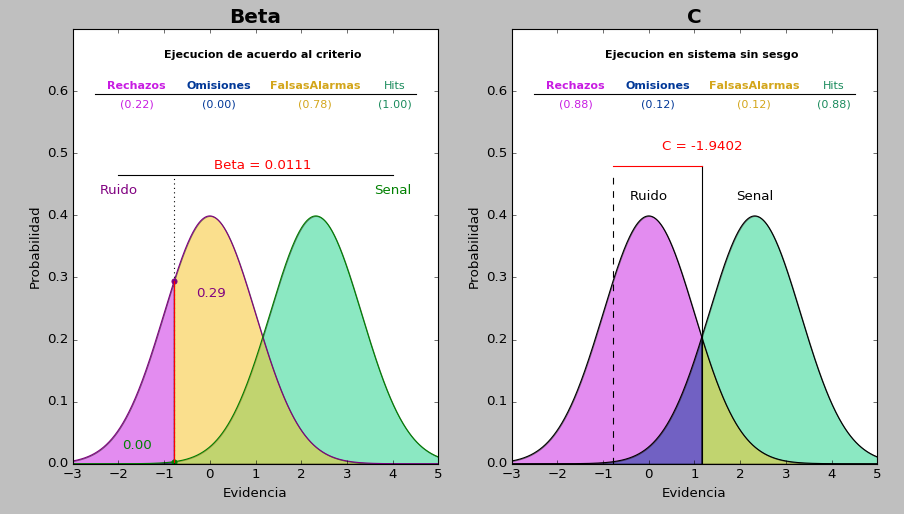
\includegraphics[width=0.60\textwidth]{Figures/Graficador_Sesgo_Liberal}\\
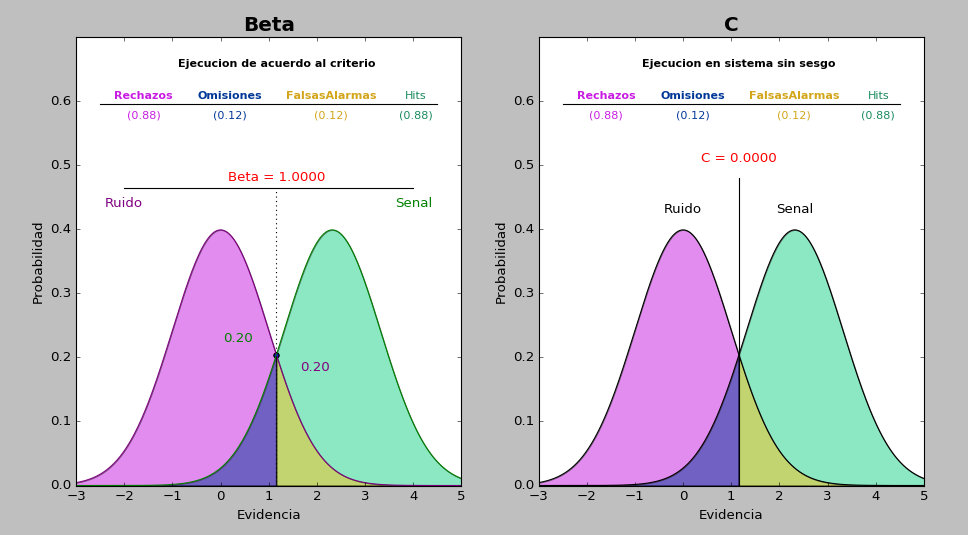
\includegraphics[width=0.60\textwidth]{Figures/Graficador_Sesgo_Neutro}\\
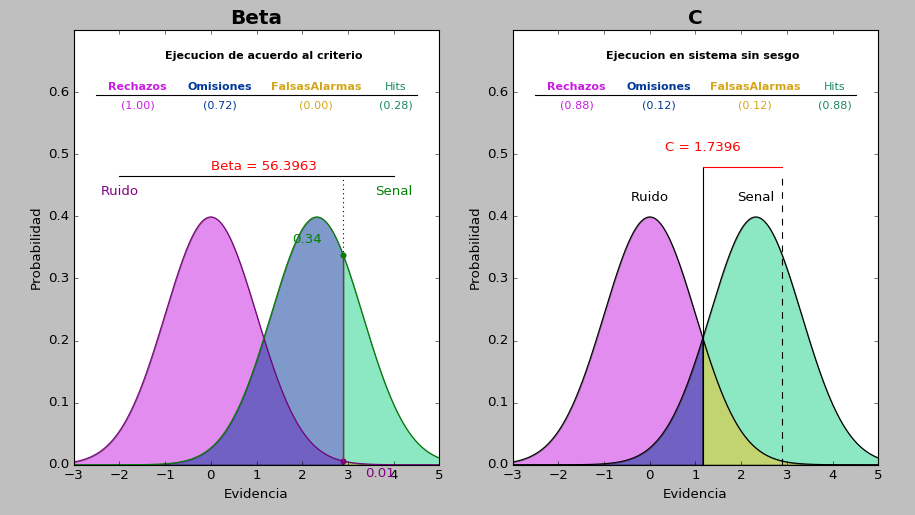
\includegraphics[width=0.60\textwidth]{Figures/Graficador_Sesgo_Conservador}\\
%\decoRule
\caption[Estimación del sesgo con base en el criterio]{La figura presenta tres capturas de pantalla de un Graficador desarrollado por parte la autora de la presente tesis, como parte de un proyecto PAPIME trabajado en el Laboratorio 25, \parencite{PAPIME}}
\label{fig:Graf_Sesgo}
\end{figure}
\end{itemize}   %Terminan los parametros

%----------------------------------------------------------------

\subsection{Curvas ROC}

Además de permitir la descripción e interpretación del desempeño observado en una tarea de detección particular con base en la estimación de los parámetros descritos, los datos obtenidos en sesiones experimentales aisladas también pueden servir para una evaluación más completa de la precisión con que el sistema evaluado podría responder a la misma tarea usando distintos criterio de elección. Las curvas ROC (identificadas así por su nombre en inglés: Receiver-Operating Characteristic curve) describen la relación entre la tasa en que las respuestas afirmativas emitidas son correctas o incorrectas -las tasas de Hits y Falsas Alarmas- en tareas de detección con cierto valor de $d'$, por cada localización posible del criterio sobre el eje de evidencia \parencite{McNicol2, Egan1959, Swets1973}.\\

La Figura~\ref{fig:Graf_ROC} ilustra la construcción de curvas ROC a partir de las tasas de ejecución reportadas en tareas de detección. En el primer panel a la izquierda, se presenta la representación gráfica (con cierta $d'$ y $k$) del desempeño observado en un caso hipotético con ciertas tasas de ejecución. En el panel intermedio, se muestra una primera aproximación al trazo de las curvas ROC, ubicando el punto de coordenadas que describe las tasas registradas de Falsas Alarmas (en el eje de las x) y Hits (en el eje de las Y). El último panel presenta la curva ROC completa para este mismo escenario (la misma $d'$) a traves de los distintos valores posibles de $k$, uniendo una serie de puntos que muestran la relación entre los Hits y Falsas alarmas que se espera observar con cada posible localización del criterio sobre el eje de evidencia.\\

\begin{figure}[th]
\centering
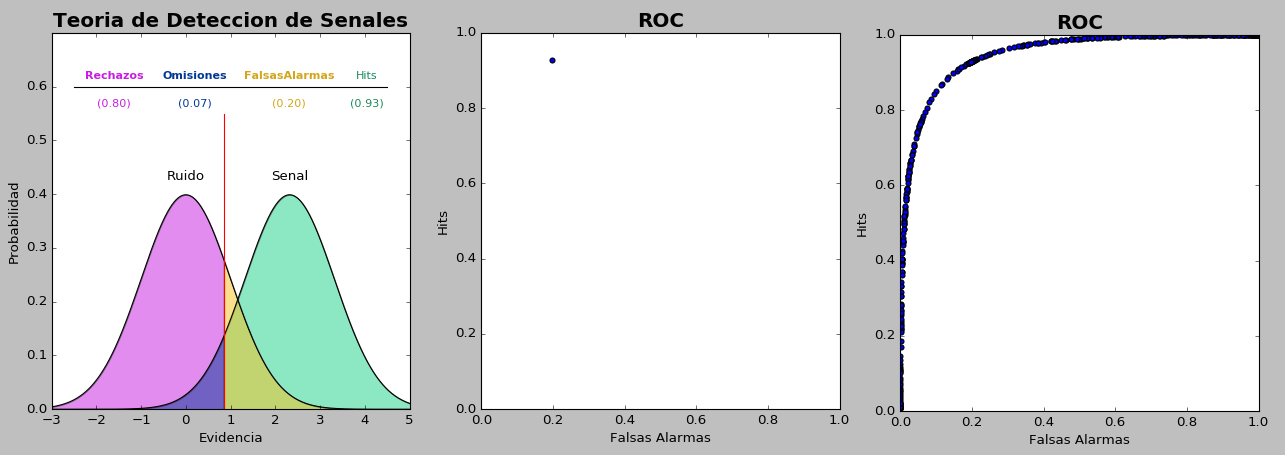
\includegraphics[width=0.90\textwidth]{Figures/Graficador_ROC12}\\
%\decoRule
\caption[Ejemplo de Curva ROC]{La figura presenta tres capturas de pantalla de un Graficador desarrollado por parte la autora de la presente tesis, como parte de un proyecto PAPIME trabajado en el Laboratorio 25, \parencite{PAPIME}}
\label{fig:Graf_ROC}
\end{figure}

Por cada valor de $d'$ se puede computar una sola curva ROC que describa los resultados esperados -en términos del intercambio entre Hits y Falsas Alarmas- para todas las posibles ubicaciones del criterio, \parencite{Tanner1954, Swets1961, Swets1973, Stainslaw1999}.\\

%Bajo el supuesto de que lo único sobre lo que el sistema detector tiene injerencia es sobre el criterio de elección a usar para emitir sus juicios de detección, y que la discriminabilidad -al ser una cualidad inherente a los estímulos comprometidos en la tarea (ya sea por la variabilidad en su presentación o percepción)- es constante y ajena a este, \\

El área bajo la curva ROC (AUC, por sus siglas en ingles: Area Under the Curve) representa una forma más precisa y completa de evaluar la sensibilidad del sistema detector ante la tarea estudiada, \parencite{Centor1985,  Stainslaw1999, McNicol5}. Nótese que se habla de "Sensibilidad" y no de "Discriminabilidad" porque, aunque ambos conceptos refieren a qué tan fácil es para el sistema distinguir entre la Señal y el Ruido y están directamente relacionados con la distancia que existe entre sus distribuciones, la primera apela a la precisión con que el sistema detector puede responder a la tarea -utilizando distintas estrategias (reglas de elección)- y la segunda hace referencia exclusivamente a una cualidad inherente a los estímulos, \parencite{Swets1973}.\\

El valor estimado de $d'$ representa la distancia entre las medias de las distribuciones y, como se mencionó anteriormente, en general se sabe que mientras más grande sea la $d'$, más fácil es la tarea para el sistema involucrado en ella. Sin embargo, es complicado interpretar el valor estimado en una tarea particular en términos de "qué tan buena" es la discriminabilidad. En otras palabras, parece poco claro qué tanto tendría que alejarse el valor de $d'$ de $0$ para afirmar que la señal es discriminable del ruido. Para ello, el trazo de las curvas ROC y el cálculo del AUC correspondiente arroja información valiosa para evaluar con qué precisión puede responder el sistema a la tarea de detección evaluada, si usara diferentes criterios, \parencite{Stainslaw1999}.\\ 

Cuando los estímulos con Señal son indistinguibles de los estímulos con Ruido ($d' = 0$), la curva ROC resultante se ve como una función de identidad que indica que al emitir un juicio de detección afirmativo, existe la misma probabilidad de que este termine siendo un Hit o una Falsa Alarma, con un AUC de 0.5 (la mitad del área total cae por debajo de la curva). Mientras mayor sea el valor de $d'$, la curva ROC resultante se alejará más de la función identidad y su AUC será cada vez más cercano a 1.0. Es decir, el AUC puede tomar valores entre 0.5 -que correspondería a un sistema que no distingue en lo absoluto entre la Señal y el Ruido- y 1.0 -que representa una distinción perfecta entre los mismos-, \parencite{Swets1973, Stainslaw1999, McNicol5}.\\

Las curvas ROC pueden ser trazadas -en teoría- a partir de un solo conjunto de tasas de ejecución \parencite{Pollack1964a, Pollack1964b, McNicol2} mediante algoritmos que asumen que el desempeño observado por parte del participante no puede "mejorar" o "empeorar" (dado que la discriminabilidad no depende de su conducta) y que se limitan a computar las Tasa de ejecución que se esperaría observar en cada ubicación posible del criterio. Sin embargo, también pueden trazarse varios puntos para guiar el trazo de la curva ROC a partir de datos obtenidos en tareas de detección donde experimentalmente se induce el uso de distintos criterios de elección por parte de los participantes, obteniendo varios conjuntos de tasas de ejecucción (varias parejas de tasas de Hits y Falsas Alarmas), \parencite{Egan1959, Swets1961, Swets1986}. Los procedimientos mediante los cuales esto se lleva a cabo se discuten a continuación.\\

%----------------------------------------------------------------

\subsection{Tareas de detección}

En cuanto a la aplicación de la TDS a la interpretación y evaluación de la ejecución de cierto tipo de participantes en cierto tipo de tareas de detección, existen tres grandes protocolos empleados para presentar la tarea y obtener datos susceptibles de ser analizados bajo el marco del modelo propuesto, \parencite{McNicol2, Stainslaw1999}. A continuación se exponen de manera general las propiedades -en términos de la información que se obtiene- y especificaciones procedimentales que caracterizan a cada uno de ellos.\\

\begin{itemize}
\item \underline{Tareas de detección binaria}\\

La forma más sencilla y estándar de presentar una tarea de detección es con un procedimiento que únicamente solicite a los participantes la emisión de juicios binarios de detección ("Sí, la señal está" o "No, no está"). Dicho protocolo se identifica en la literatura con el nombre de "tareas de detección binaria" o "tareas Sí/No", \parencite{McNicol2}.\\

Las tareas Sí/No realizadas en el laboratorio consisten en la presentación aleatoria de una serie de ensayos (N) compuesta por ensayos que contienen la señal (S) y ensayos con sólo ruido (R), siendo la única respuesta que los participantes deben registrar en cada ensayo si la señal estuvo presente o no. Típicamente, la cantidad de ensayos S y R presentados durante la tarea es la misma. Esto es recomendable por dos grandes razones: 1) Garantiza que las tasas de Hits y Omisiones sean tan representativas del desempeño del participante a lo largo de la tarea experimental como las tasas de Falsas alarmas y Rechazos correctos, pues se tienen la mismma cantidad de oportunidades de cometer cada tipo de acierto y error, y 2) Evita que el sistema evaluado desarrolle un sesgo a favor de una respuesta particular en función a cuál sea el tipo de ensayo que más se le presenta, \parencite{Nevin1969, Wickens}.\\

Por cada tarea 'Sí/No' conducida, se obtiene un set de tasas de ejecución que permiten trazar uno solo de los puntos que componen la curva ROC que describiría la sensibilidad del sistema evaluado. Así que, para obtener más datos con los cuales trazar la curva (más puntos que representen un conjunto de tasas de ejecución), tendría que correrse la misma tarea más de una vez, con los mismos estímulos y en los mismos participantes, pero incitando el uso de distintos criterios de elección en cada ocasión. Esto último se puede hacer de manera explícita (solicitándole al participante que sea más o menos estricto en la emisión de sus respuestas), o implícita (presentando la tarea con diversas matrices de pago que promuevan que el participante evite un cierto tipo de error o busque aumentar cierto tipo de acierto), \parencite{Wickens, McNicol2}.\\

Un problema evidente con el trazo de curvas ROC a partir de los datos obtenidos en tareas de detección binarias repetidas es que se requiere un número considerable de repeticiones que deben estar compuestas por el mismo número de ensayos. Exponer a un mismo participante a la misma tarea y los mismos estímulos tantas veces trae consigo el riesgo de que su desempeño se vea afectado por la fatigua o el aprendizaje. Si este fuera el caso, los datos obtenidos no sólo serían reflejo de cambios en el criterio usado para responder a la tarea, sino que también podría haberse alterado la propia discriminabilidad de la tarea (el aprendizaje puede hacer que los participantes se vuelvan mejores distinguiendo entre la Señal y el Ruido, y la fatiga, tener el efecto opuesto). Esto representa un problema porque entonces, la curva ROC trazada no representaría la sensibilidad del sistema evaluado ante "una misma" tarea, ya que se estaría violando el supuesto fundamental de que la discriminabilidad es constante, \parencite{McNicol2}.\\

\item \underline{Tareas con escala de confianza}\\

Una segunda forma de presentar la tarea de detección -que puede ser entendida como una extensión del protocodo con tareas Sí/No-, es solicitando a los participantes que respondan a la misma valorando y asignando un puntaje que represente la certeza que tienen sobre la pertenencia de cada estímulo presentado a las categorías Señal o Ruido.\\

En términos del procedimiento, las tareas de detección binarias y con escala de confianza son idénticas: se muestra a los participantes una serie de ensayos (N) dentro de la cual se presentan de manera aleatoria ensayos con la señal (S) y ensayos con sólo Ruido (R), solicitándoles que registren una respuesta al término de cada ensayo. La única diferencia entre ambos protocolos es el tipo de respuesta solicitada -y en consecuencia, la robustez de las estimaciones que pueden hacerse sobre la sensibilidad del sistema-. En tareas "Sí/No" los participantes emiten una de dos posibles respuestas mutuamente excluyentes; y en tareas con Escala de confianza, se asigna a cada estímulo evaluado un puntaje dentro de una Escala particular con cierto número de opciones de respuesta, \parencite{Stainslaw1999}.\\

Existen varias formas en que puede presentarse la Escala de Confianza, \parencite{McNicol2}. Por ejemplo, una de ellas podría ser solicitando que se responda de acuerdo a la confianza que se tendría en asignar cada estímulo evaluado a la categoria Señal (donde los valores más altos serían asignados a los estímulos que que se encuentren más hacia la derecha en el eje de las evidencias y los valores bajos a los estímulos más a la izquierda, que podrían haber ser identificados como Ruido); una segunda forma, sería distinguiendo entre la certeza que se tiene sobre que el estímulo evaluado sea una Señal o Ruido, (los valores más altos reflejan la confianza que se tiene en que se trate de una Señal y los valores más bajos, a la certeza de que se trate de Ruido). Como se presenta en la tabla incluída en la parte superior de la Figura~\ref{fig:Conf_Rat}, ambas formas de presentar la escala proporcionan -en teoría- la misma información y, en general, la elección de una u otra depende del experimentador.\\

El supuesto detras de la interpretación de los puntajes de confianza registrados, es que los participantes fijan un criterio sobre el eje de evidencia por cada opción de respuesta en la Escala de Confianza que va a determinar cuál de estas se emite. Es decir, se asume que el puntaje asignado en cada ensayo depende de cuál es el último criterio de elección que la evidencia juzgada rebasa, \parencite{McNicol2}. La Figura~\ref{fig:Conf_Rat} ilustra esta idea: en la parte superior se presenta una escala de confianza de 6 elementos (se ejemplifican las dos formas -previamente expuestas- en que puede ser presentada), y en la parte inferior, la representación gráfica del modelo de detección de señales.\\

\begin{figure}[th]
\centering
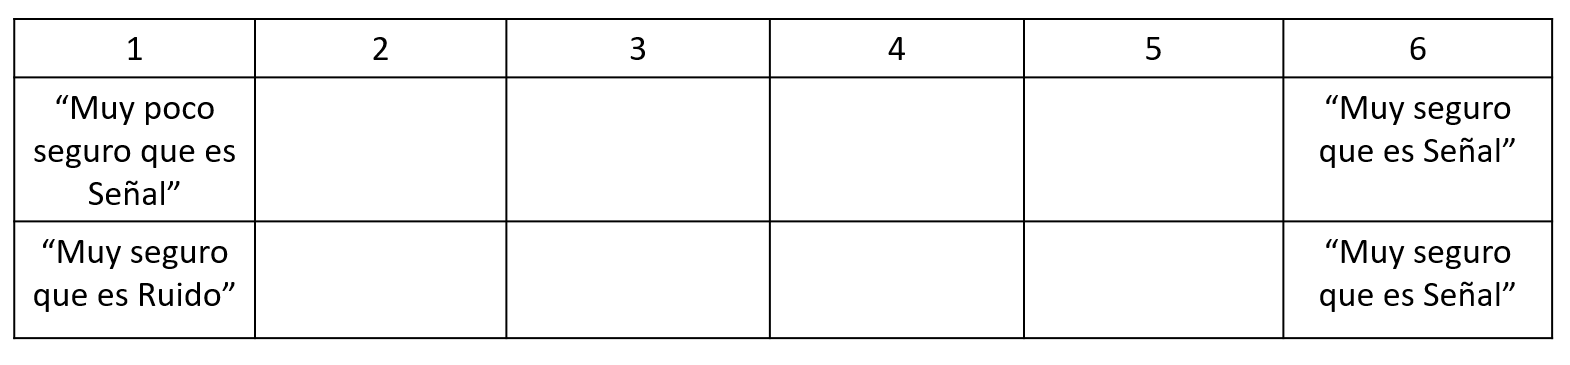
\includegraphics[width=0.80\textwidth]{Figures/Puntajes_Criterios}\\
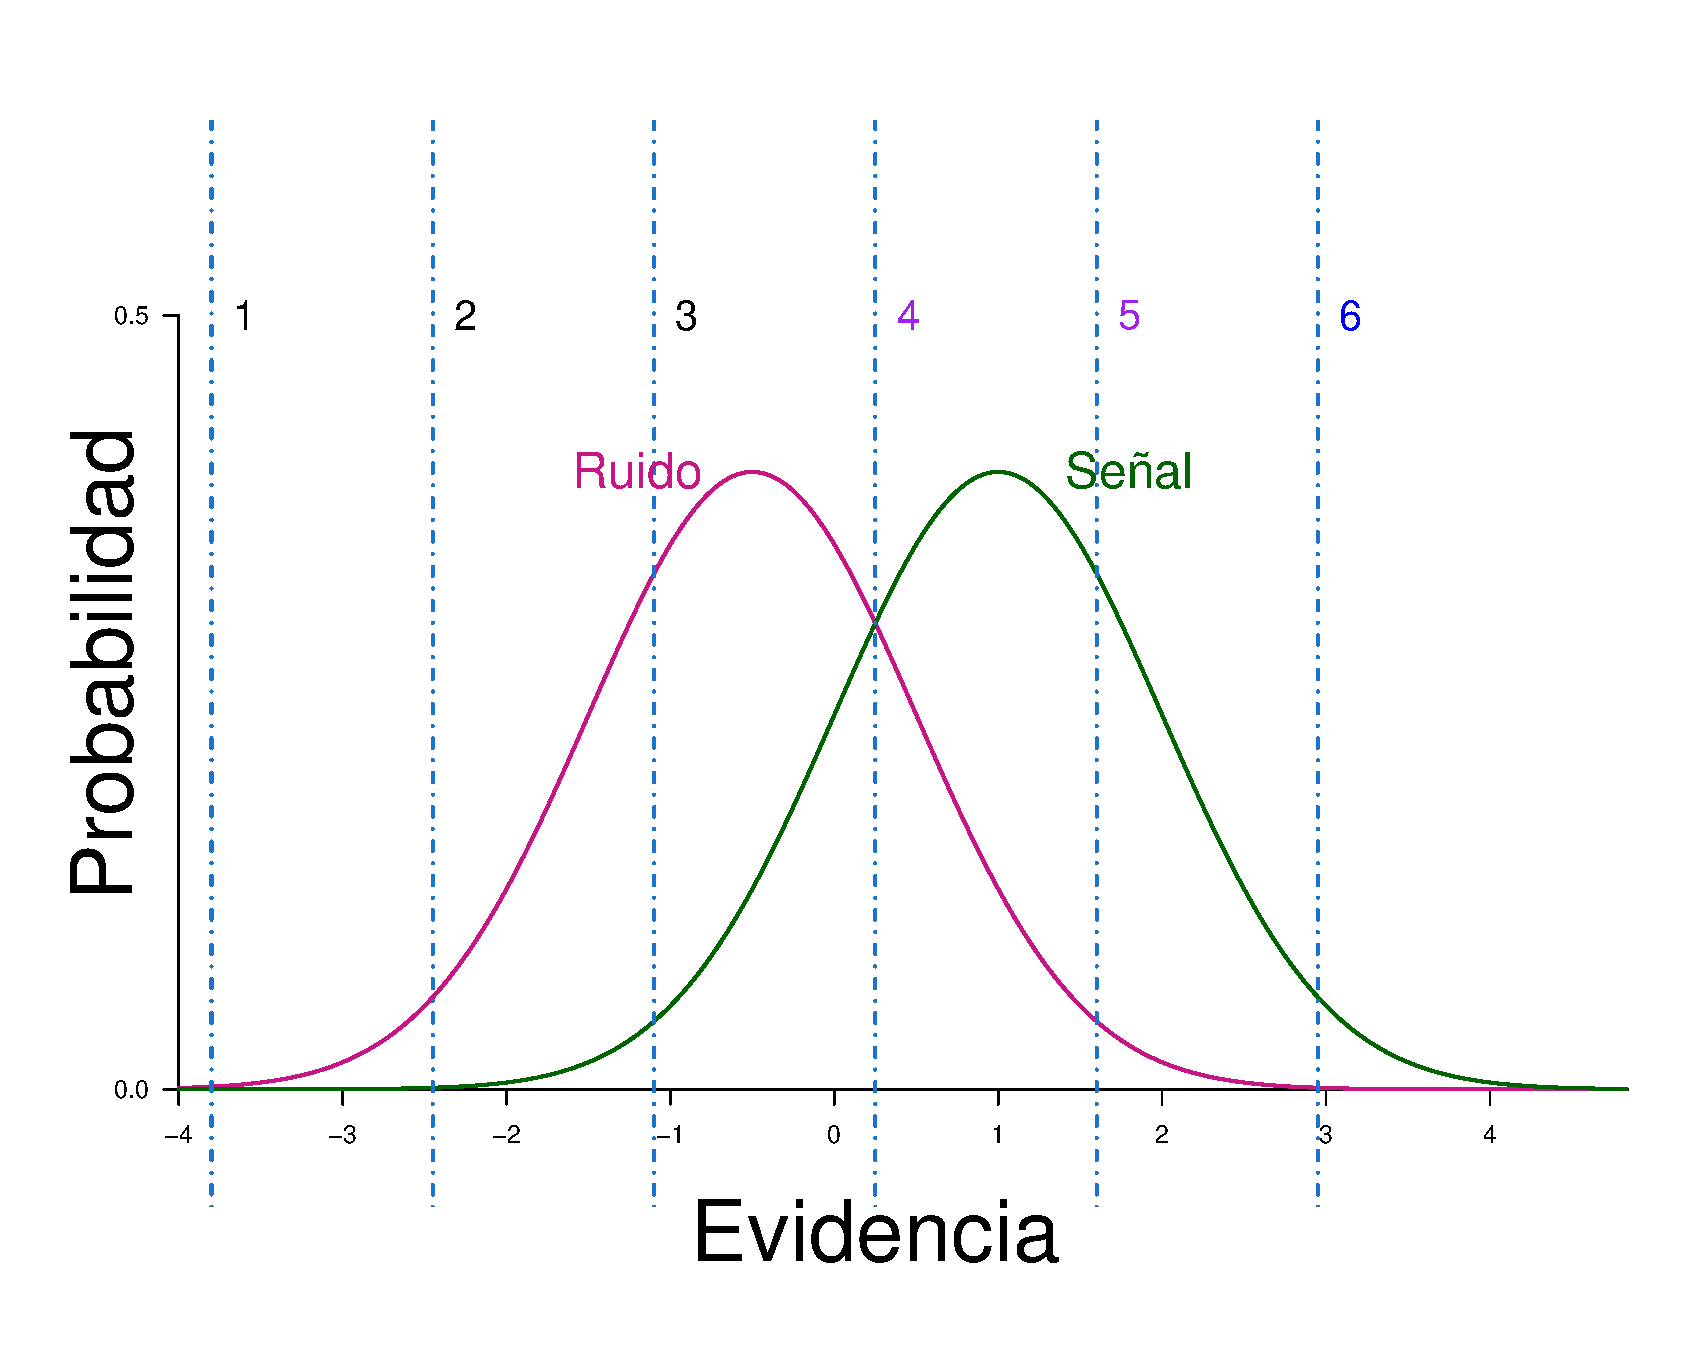
\includegraphics[width=0.70\textwidth]{Figures/ConfidenceRating}\\
%\decoRule
\caption[Ejemplo ]{}
\label{fig:Conf_Rat}
\end{figure}


El protocolo de Escala de Confianza permite -en un mismo experimento- recoger datos que representen el uso de criterios múltiples (tantos como opciones de respuesta se le proporcionen) por parte del sistema detector en una misma tarea de detección, permitiéndonos asumir que la discriminabilidad se mantiene constante. Es por ello, que el uso de Escala de Confianzas $n$ opciones de respuesta, provee una forma sencilla y directa de obtener datos suficientes para trazar puntos ($n - 1$) que permitan formar la curva ROC que represente la sensibilidad del sistema, \parencite{Stainslaw1999, McNicol2, McNicol5}.\\ 

Idealmente, se espera que el participante utilice todas las opciones de respuesta incluídas en la Escala de confianza. Esto se puede conseguir de manera explícita o implícita; solicitando a los participantes que lo hagan así, o bien, modificando el número de puntajes incluídos en la Escala. En general, se recomienda que la Escala esté compuesta por un número par de opciones de respuestas que oscile entre 4 y 10 \parencite{McNicol2, McNicol5}. Esto con el fin de evitar que los participantes elijan la opción intermedia siempre que se sientan inseguros sobre su respuesta.\\

\item \underline{Tarea de Elección forzada}\\

Existe un tercer protocolo bajo el cual se presentan las tareas de detección, identificado como tareas de Elección forzada entre $m$ alternativas, donde se presentan simultáneamente $m - 1$ estímulos que contienen sólo ruido y $1$ con señal. La tarea del participante consiste en identificar la Señal dentro del conjunto de estímulos que se le presentan, \parencite{Stainslaw1999}. En general, se asume que cada estímulo presentado contiene cierto valor de evidencia -cierta ubicación en el eje sobre el cual se despliegan las distribuciones- que el participante compara para elegir como 'Señal' aquel que tenga un valor mayor -de acuerdo con el supuesto de que en general, los valores de la distribución Señal caen por encima del Ruido-, \parencite{McNicol2}.\\

Dada la relación que representan, el área bajo la curva ROC trazada con un protocolo de preguntas binarias o con Escala de confianza puede interpretarse como la proporción de veces que el participante cuyo desempeño se describe, podría identificar correctamente la Señal, si esta fuera presentada simultáneamente junto con el Ruido. A su vez, la proporción de respuestas correctas obtenidas a lo largo de una tarea de Elección forzada proporciona una medida de la sesibilidad del sistema, independiente del sesgo del sistema. Dicha medida -al igual que el AUC-, tendría que variar entre el azar ($\frac{1}{m}$) y el desempeño perfecto ($1.0$), \parencite{Stainslaw1999}.\\
\end{itemize}


















\section{Teoría de Detección de Señales en Memoria}

La Teoría de Detección de Señales ha sido ampliamente utilizada en distitnas áreas de la Psicología Experimental tanto como un marco de referencia conceptual para pensar en diversas situaciones de detección, como herramienta de análisis de datos obtenidos en este tipo de tareas. Una de estas áreas la constituye el estudio de la Memoria, donde se han aterrizado los supuestos y conceptos desarrollados originalmente en la TDS para el estudio del aprendizaje humano, la retención y el reconocimiento de ciertos elementos estudiados, \parencite{Murdock1965, Bernbach1967, Banks1970, White1999}.\\

Al diseñar las tareas presentadas en estudios de Memoria como instancias de un problema de detección, los resultados obtenidos se pueden clasificar de acuerdo a las mismas categorías señaladas en cada celda de la matriz que se presenta en la Figura~\ref{fig:Mat_Output}, dependiendo la correspondencia que exista entre la respuesta registrada por los participantes y el tipo de ensayo presentado. Y de la misma forma, las tasas de Hits y Falsas Alarmas registradas para la localización de los criterios evaluados (en tareas Sí/No que inducen distintos sesgos, o mediante el uso de escalas de confianza) pueden emplearse para trazar curvas ROC \parencite{Egan1958}, también llamadas curvas MOC (por sus siglas en inglés "Memory Operant Curve") para enfatizar su adscripción al estudio de la Memoria, \parencite{Norman1965, KintschCarlson1967}.\\

La aplicación de la TDS al estudio de la Memoria ha impactado en el desarrollo de este útlimo en términos de cuatro grandes ejes \parencite{Banks1970}, que son:\\

\begin{enumerate}
\item La noción de la "Fuerza de Memoria".\\

Aceptar la TDS como marco para la descripción de tareas en Memoria implica asumir que el "input" con base en el cual los participantes emiten sus respuestas ensayo a ensayo son valores $x$ que corresponden a distintos puntos del eje de evidencia sobre el cual se despliegan las distribuciones de Ruido (los estímulos distractores) y Señal (los estímulos a identificar de acuerdo al procedimiento empleado). Es decir, el desempeño observado se interpreta como resultado de la interacción entre la "fuerza de memoria" evaluada en cada ensayo y un proceso de decisión que determina cuándo esta es lo suficientemente grande para juzgar la pertenencia de ciertos estímulos a la categoría Señal. En términos de la exploración de este supuesto y sus implicaciones, resaltan los trabajos orientados a evaluar la naturaleza de la "fuerza de memoria" desplegada sobre el eje de evidencia (por ejemplo, si puede entenderse como una serie de valores contínuos o discretos), y a estudiar su interacción con algunos de los procesos propios de la Memoria (por ejemplo, el estudio, la retención y el olvido), \parencite{Bernbach1967, Wickelgren1966, Parks1966}.\\

\item La noción del Criterio de Elección como opuesta a los Umbrales de respuesta.\\

Una de las ventajas más evidentes de la aplicación de la TDS al estudio de la memoria es que permite entender los Falsos Positivos en términos de una confusión entre la evidencia -la "fuerza de memoria", también llamada "familiaridad", "grado de empate" o "relacionabilidad"- producida por el Ruido y la Señal (el sobrelape entre las distribuciones), en vez de asumir que los participantes responden de manera aleatoria a los ensayos donde se presentan los estímulos distractores. En otras palabras, pensar este tipo de situaciones en términos de un modelo de detección de señales como el propuesto por la TDS permite abandonar la noción originalmente planteada por la Teoría del Umbral de que existe tal cosa como un "umbral de estimulación" que debe ser rebasado para que el sistema sea capaz de identificar la pertenencia de los estímulos a una u otra categoria, \parencite{Yonelinas1996}.\\
 
\item La noción de que existen distribuciones subyacentes (y la definición de sus características).\\

Como se mencionó previamente, los datos obtenidos en experimentos de memoria (Verdaderos Positivos y Falsos positivos, o bien, Hits y Falsas Alarmas) pueden utilizarse para construir curvas MOC que describan la sensibilidad de los participantes al discriminar los estímulos distractores de los estímulos previamente estudiados, mediante el uso de distintos criterios de elección. A su vez, dado que cada curva MOC representa un valor fijo de $d'$, las curvas obtenidas sirven como punto de referencia para evaluar el tipo de distribución que permitiría explicar mejor la relación observada entre Hits y Falsas Alarmas y sus características particulares, \parencite{Kintsch1967, Ratcliff1992, Ratcliff1994}.\\

\item Análisis de datos y descripción del desempeño de los participantes.\\

Finalmente, se encuentran los trabajos que se limitan a utilizar la TDS como una herramienta para interpretar los datos obtenidos en estudios de memoria que incorporan la metodología asociada con las tareas de detección, \parencite{Marks1964, Wickelgren1966_Solo, Schulman1967}.\\
\end{enumerate} 

\subsection{ Memoria de Reconocimiento}

Dentro del campo de estudio de la Memoria, una de las sub-áreas donde la aplicación de la TDS parece ser más directa y evidente es el de la Memoria de Reconocimiento \parencite{Parks1966}. Bajo este esquema, las tareas de reconocimiento se definen como instancias de una tarea de detección en donde los participantes tienen que indicar cuáles de los elementos presentados en una lista se le habían mostrado en una fase previa (los "estímulos viejos": las señales) y cuáles no (los "estímulos nuevos": el ruido), \parencite{Bernbach1967, Kintsch1967}.\\

Aplicar la TDS al estudio de la Memoria de Reconocimiento implica asumir que existe tal cosa como una 'fuerza de memoria' ('memory strength', en inglés) que refleja el grado en que un estímulo cualquiera es percibido como 'familiar' para el sistema que busca emitir un juicio de detección -o en este caso, de reconocimiento-. La fuerza de memoria evocada por cada estímulo se compara con un criterio de elección para que el sistema pueda decidir si lo reconoce, o no, como 'elemento antes visto'.\\ 

\begin{figure}[th]
\centering
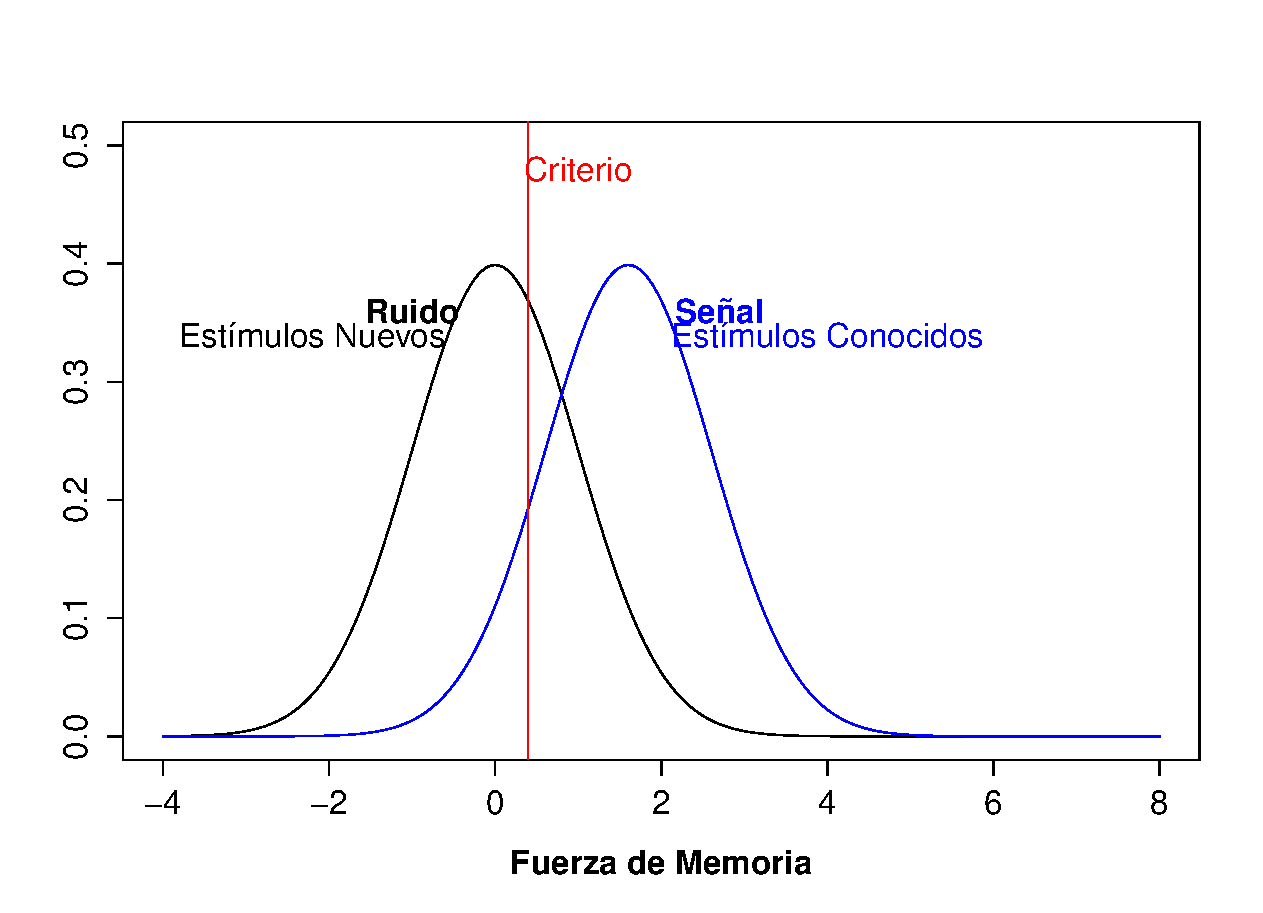
\includegraphics[width=0.60\textwidth]{Figures/RM_SDT_1} 
\decoRule
\caption[SDT en Memoria de Reconocimiento]{Modelo de Detección de Señales aplicado al estudio de Memoria de Reconocimiento}
\label{fig:RM_SDT_1}
\end{figure}

La Figura~\ref{fig:RM_SDT_1} ilustra la forma en que los supuestos y conceptos básicos de la TDS se aplican al contexto de la Memoria de Reconocimiento. La Señal a detectar son los estímulos ya conocidos (típicamente referidos como "estímulos viejos") y el Ruido se compone por los estímulos nuevos, asumiendo que éstos pueden -o no- ser confundidos con los primeros; el 'eje de evidencia' a lo largo del cual se despliegan las distribuciones de Ruido y Señal, se convierte en un 'eje de familiaridad' que representa lo que podría entenderse como 'fuerza de memoria'. Al igual que en la TDS clásica, se espera que los estímulos pertenecientes a la distribución Señal tengan valores más altos de 'familiaridad' que aquellos nunca antes vistos, admitiendo la posibilidad de que éstos puedan llegar a producir la misma evidencia y confundirse con los estímulos viejos. Por último, se incorpora la idea de que la emisión de juicios de reconocimiento depende de la comparación de la 'familiaridad' de cada estímulo con un criterio de elección.\\

Las tareas de reconocimiento conducidas en el laboratorio suelen componerse de dos fases, \parencite{Ratcliff1992}. En la primera ("la fase de estudio") se presenta a los participantes una serie de elementos para que los estudien de manera intencional (solcitándoles explícitamente que las estudien para su reconocimiento posterior) o incidental (planteándoles alguna tarea distractora que obligue a los participantes a interactuar con ellos) \parencite{Noldy1990}. En la segunda fase ("la fase experimental" o "de reconocimiento") se presentan los mismos elementos incluidos en la primera fase, más una cantidad igual de elementos nunca antes presentados, y se encomienda a los participantes la tarea de identificar cuáles de los elementos incluidos en esta segunda fase son "viejos" o "nuevos".\\









Una de las regularidades particulares en la aplicación de la TDS al estudio de la Memoria de Reconocimiento tiene que ver con las inferencias realizadas a partir del trazo de las curvas ROC con los datos obtenidos en este tipo de tareas \parencite{VanZ2000, Ratcliff1992, Ratcliff1994}, acerca de las distribuciones subyacentes. 

Como se mencionó en el Capítulo 1, la TDS en su forma típica define las distribuciones de ruido y señal como distribuciones Gaussianas con varianzas iguales (i.e. con una misma desviación estándar). A propósito de ello, podemos hablar de una particularidad que tiene la aplicaicón de la TDS a estudios de memoria de reconocimiento, que ha sido constante y consistentemente demostrada con los datos: la distribución de Estímulos Viejos suele mostrar mayor desviación estándar que la distribución de Ruido, justo como se muestra en la Figura~\ref{fig:RM_SDT_2}.\\


\begin{figure}[th]
\centering
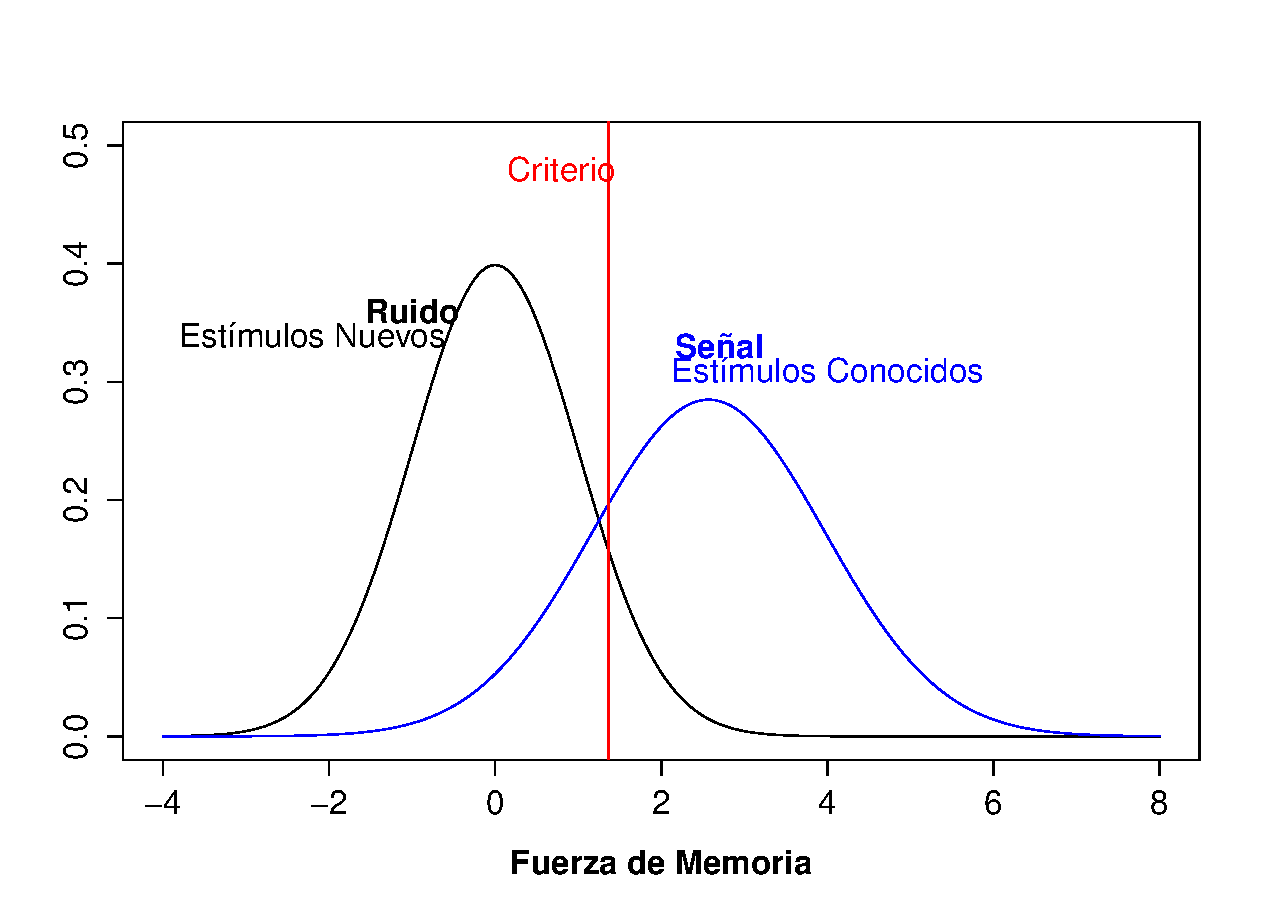
\includegraphics[width=0.60\textwidth]{Figures/RM_SDT_2} 
\decoRule
\caption[SDT en Memoria de Reconocimiento (Varianzas Desiguales)]{Modelo de Detección de Señales con varianzas desiguales aplicado al estudio de Memoria de Reconocimiento}
\label{fig:RM_SDT_2}
\end{figure}


\subsection{Implicaciones y conflictos}




\parencite{Wixted2007}

La Teoría del Procesamiento Dual (TPD; o PDT por sus siglas en inglés) sostiene que existen dos procesos fundamentales involucrados en todo juicio de reconocimiento: la recolección y el análisis de familiaridad. El primero corresponde a la extracción de rasgos y detalles específicos del estímulo a evaluar, (i.e. el estímulo que queremos determinar si se ha visto antes, o no), un proceso que requiere cierto tiempo; el segundo, es entendido como un fenómeno más o menos automático y casi instantáneo donde el sistema identifica el estímulo como 'familiar' y decide que lo ha reconocido de alguna experiencia previa. 

Una de las principales críticas que devienen de la aplicación de la TDS al estudio de la Memoria de Reconocimiento, es que ello implica que el organismo fija un criterio de elección a lo largo de un eje de evidencia -comúnmente identificado como 'familiaridad'-.   \parencite{Brown1977}

























\section{El Efecto Espejo}

El 'Efecto Espejo' refiere a un patrón de respuestas reportado consistentemente en estudios de Memoria de Reconocimiento donde se compara el desempeño de los participantes entre dos clases de estímulos, que difieren en la precisión con que sus estímulos son reconocidos (diferentes valores de $d'$), bajo el marco de la TDS, \parencite{Glanzer1993}. En dichos experimentos, se ha encontrado evidencia sólida de que la diferencia en la discriminabilidad de los elementos 'nuevos' y 'viejos' que conforman cada clase de éstímulos, se presenta tanto en términos de una mayor precisión identificando los estímulos viejos como 'viejos' (más Hits), como en la identificación de los estímulos nuevos como 'no viejos' (menos Falsas Alarmas). Es decir, las diferencias en $d'$ se ven reflejadas no sólamente en una mayor cantidad de aciertos, sino también, en una reducción de errores.\\

La diferencia entre la proporción de Hits y Falsas Alarmas reportada entre dos clases de estímulo a comparar en tareas de reconocimiento (estímulos A, que son fácilmente reconocibles y estímulos B, que se reconocen con mayor dificultad) analizadas bajo el marco de la TDS, sugiere que existen cuatro distribuciones que subyacen a la presentación de los estímulos y el orden en que se despliegan las distribuciones de estímulos 'viejos' A y B, es el inverso del orden en que se presentan sus respectivas distribuciones de estímulos 'nuevos', \parencite{Glanzer1990, DeCarlo2007}. La representación gráfica de este orden (Nuevos(A), Nuevos(B), Viejos(B) y Viejos(A)), se presenta en la Figura~\ref{fig:Ejem_EfectoEspejo}. La peculiaridad con que las distribuciones de ruido y señal parecen "reflejarse" entre clases de estímulos, es la razón por la cual se ha identificado a dichos patrones de respuesta bajo el nombre de Efecto Espejo.\\

\begin{figure}[th]
\centering
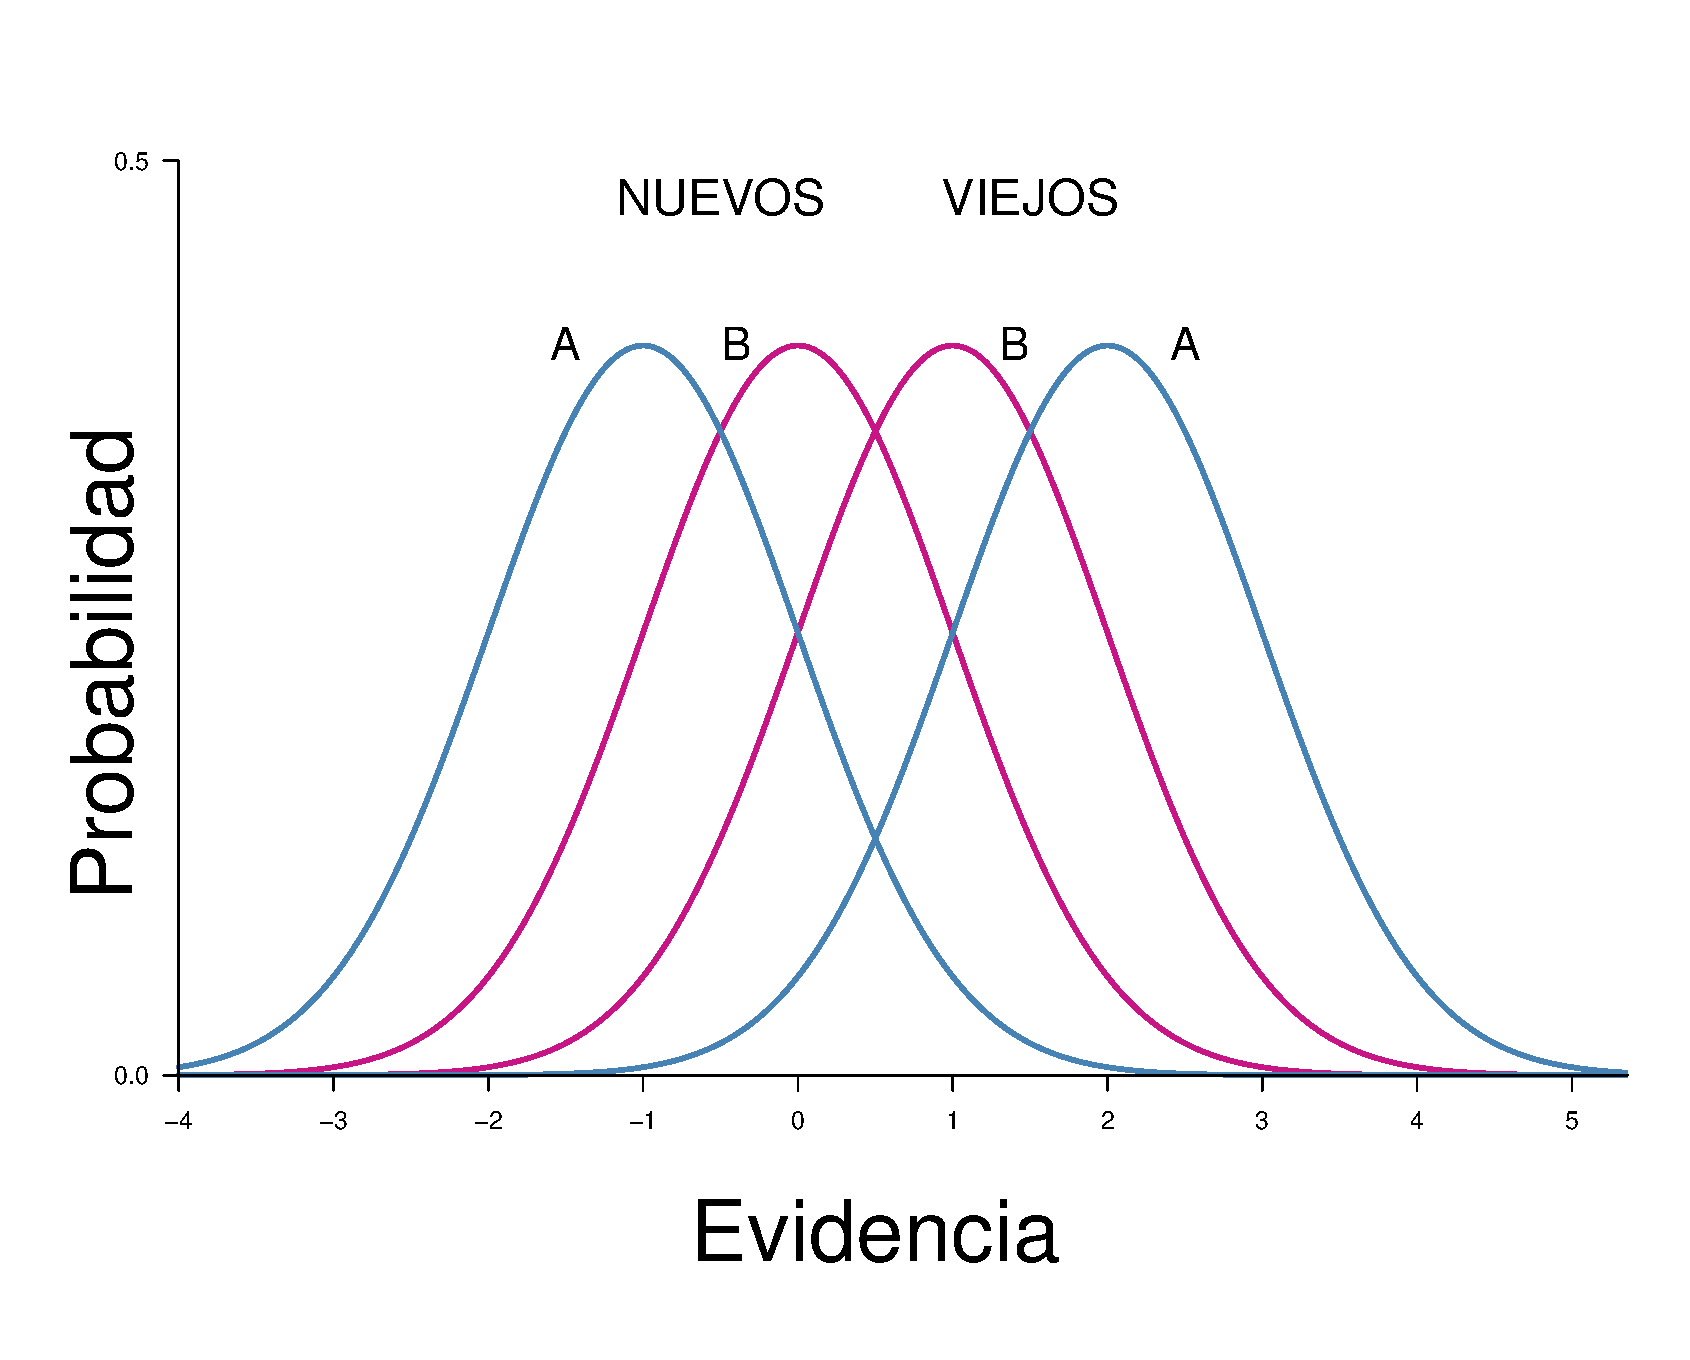
\includegraphics[width=0.7\textwidth]{Figures/EfectoEspejo}
%\decoRule
\caption[Representación gráfica del Efecto Espejo]{}
\label{fig:Ejem_EfectoEspejo}
\end{figure}

La evidencia en favor del Efecto Espejo en experimentos de Memoria de Reconocimiento se reporta a lo largo de una amplia variedad de "clases de estímulos" y en distintos protocolos de presentación de tareas de detección (Preguntas Sí/No; Escala de Confianza y Elección Forzada de dos alternativas), \parencite{Glanzer1990}, en estudios que cumplen las siguientes condiciones:\\

\begin{itemize}
\item Existen al menos dos clases de estímulos -típicamente identificados con las letras A y B-, entre los cuales se busca comparar el desempeño de los participantes, y que difieren en su nivel de discriminabilidad. En otras palabras, existe una clase de estímulos (A) que se caracteriza porque está compuesto de estímulos que se reconocen con mayor facilidad al ser presentados en más de una ocasión que la segunda clase de estímulos (B) incluida en el procedimiento.\\

\item Los estímulos que componen las clases A y B se presentan de manera simultánea y aleatoria durante la tarea, tanto en la fase de entrenamiento (cuando los estímulos que más adelante serán identificados como 'viejos' se presentan por primera vez), como en la fase de reconocimiento; sin que los participantes tengan forma de saber que se le está presentando más de un tipo de estímulo, (y más aún,  que su desempeño se va a evaluar en términos de las diferencia con que responda a cada uno de estos). Esto se hace por dos razones: 1) permite asumir que el participante está respondiendo con base en un sólo criterio de elección y 2) provee cierta garantía sobre la forma en que las distribuciones subyacentes están escaladas, \parencite{DeCarlo2007}.\\
\end{itemize}

La separación que se observa en la Figura~\ref{fig:Ejem_EfectoEspejo} entre las distribuciones de estímulos viejos A y B (las distribuciones de las señales a detectar o, en este caso, "reconocer") tiene sentido bajo el supuesto de que las tareas de reconocimiento funcionan como una instancia de detección de señales y se espera que exista una mayor distancia entre la distribución señal cuyos estímulos se reconocen con mayor precisión (Vieja(A)) y el Ruido. Sin embargo, no existe razón para esperar que dicha diferencia se "refleje" y aparezca también en las distribuciones de estímulos nuevos. En el contexto del estudio de la Memoria de Reconocimiento, no habría por qué esperar que el desempeño de los participantes entre los estímulos nuevos A y B (el ruido), puesto que en cualquier caso se trata de  estímulos que no han sido mostrado previamente y no habría forma de explicar las discrepancias sugeridas por el Efecto Espejo entérminos de su "familiaridad", \parencite{Glanzer1993}. Esta y otras complicaciones e implicaciones arrojadas por el Efecto Espejo y su consistencia, se describen con detalle más adelante.\\

\subsection{Evidencia recolectada}

Como se mencionó previamente, la evidencia en favor de la prevalencia del Efecto Espejo en tareas de Memoria de Reconocimiento analizadas bajo el marco de la TDS, donde se compara la ejecución de los participantes entre clases de estímulos que difieren en su nivel de discriminabilidad, se presenta de manera consistente en los datos obtenidos a traves de distintos protocolos experimentales. \parencite{Glanzer1990, Glanzer1993}. Los patrones de respuesta identificados en cada caso y su relación con el Efecto Espejo (y su representación gráfica presentada en la Figura~\ref{fig:Ejem_EfectoEspejo}) se exponen a detalle a continuación:\\

\begin{itemize}
\item \underline{Efecto Espejo en Tareas Sí/No}\\

En el caso de las tareas binarias "Sí/No", donde de manera aleatoria se presenta a los participantes estímulos nuevos y viejos de ambas clases de estímulos durante la fase de reconocimiento para que este emita una respuesta binaria "Sí/No" para señalar si se trata de un estímulo que le fue presentado con anterioridad (estímulo viejo; la señal), o no (estímulo nuevo; el ruido), se reporta el siguiente patrón de respuestas:\\

\begin{center}
$p[Si(NuevoA)] < p[Si(NuevoB)] < p[Si(ViejoB)] < p[Si(ViejoA)]$\\
\end{center}
\begin{center}
donde $p[Si]$ es la proporción de juicios de reconocimiento afirmativos ("Sí, este estímulo se me había presentado antes"), $A y B$ son las clases de estímulo empleadas y $Nuevo y Viejo$ señala la pertenencia de los estímulos presentados a la categoría Ruido o Señal, respectivamente, \parencite{Glanzer1993}.\\
\end{center}

De acuerdo con la correspondencia entre la emisión de juicios de reconocimiento afirmativos y el tipo de estímulo presentado, la relación anteriormente descrita también puede definirse en términos de Hits y Falsas Alarmas:\\

\begin{center}
$F.Alarmas(A) < F.Alarmas(B) < Hits(B) < Hits(A)$\\
\end{center}
\begin{center}
donde $F.Alarmas$ y $Hits$ refieren a la tasa de Hits y Falsas Alarmas observadas durante la tarea, para cada una de las clases de estímulos, \parencite{Glanzer1993}.\\
\end{center}

De acuerdo con su interpretación clásica en el marco de la TDS, en este tipo de experimentos se asume que los participantes están emitiendo sus juicios de detección con base en la comparación de la evidencia evaluada -en este caso, el grado de familiaridad- momento a momento y un criterio de elección, que va a determinar si ésta es suficiente para juzgar su pertenencia a la categoría Señal ("Sí, ya había visto este estímulo antes"). Dado que los participantes no saben que su desempeño se comparará entre dos clases de estímulos diferentes -o si quiera que se le están presentando "clases" de estímulos diferentes-, los Hits y Falsas Alarmas registrados se interpretan como el reflejo de un sólo criterio de elección \parencite{Glanzer1993}, que cruza las cuatro distribuciones involucradas en un mismo punto (ver Figura~\ref{fig:Ejem_Espejo_YesNo}).\\

\begin{figure}[th]
\centering
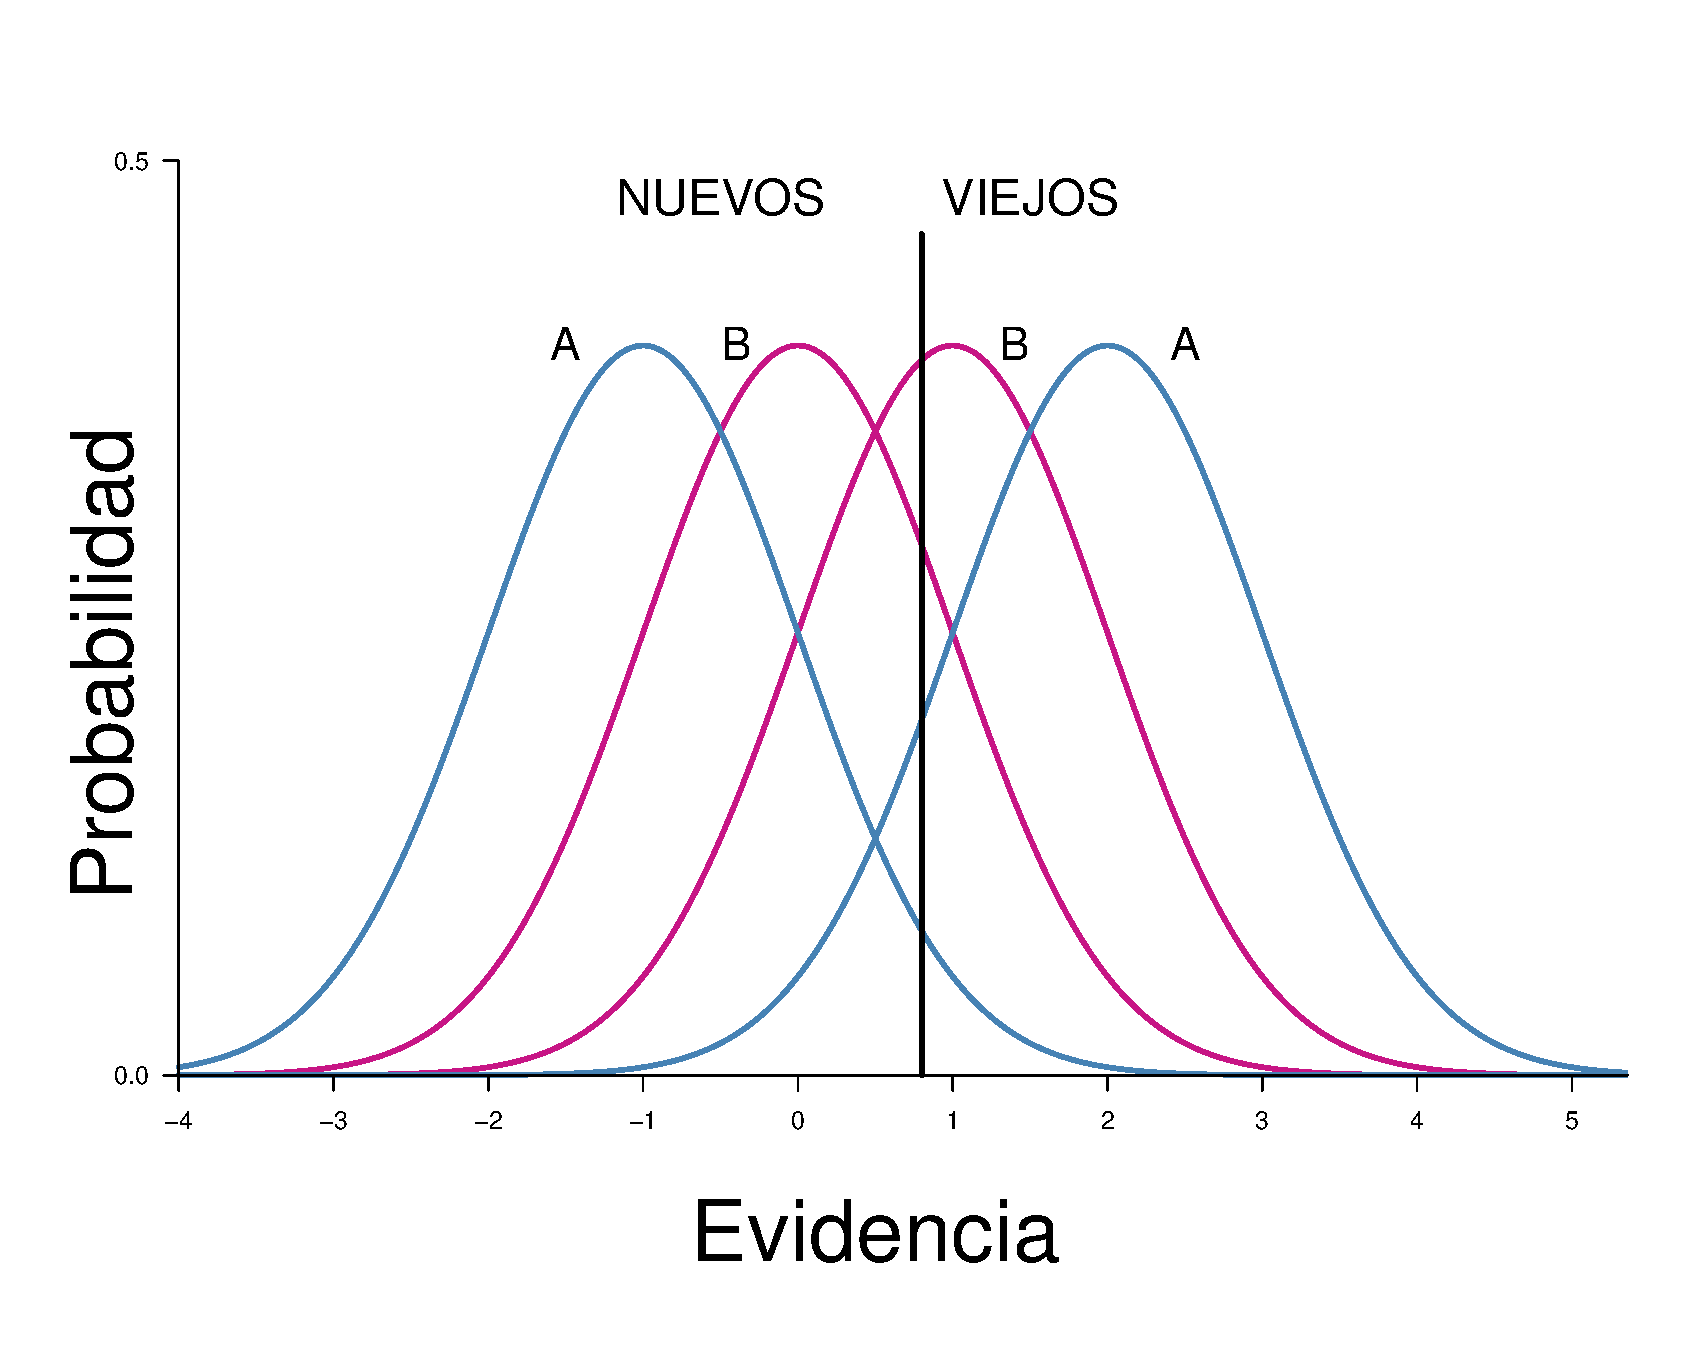
\includegraphics[width=0.7\textwidth]{Figures/EfectoEspejo_YesNo}
%\decoRule
\caption[Representación gráfica del Efecto Espejo]{}
\label{fig:Ejem_Espejo_YesNo}
\end{figure}

La ubicación y órden de las cuatro distribuciones presentadas en la Figura~\ref{fig:Ejem_Espejo_YesNo} se infiere siguiendo la misma lógica que en la estimación clásica de parámetros de la TDS con un solo conjunto de Señal y Ruido descrito previamente. En otras palabras, las tasas reportadas de Falsas Alarmas y Hits A y B reflejan el área de las distribuciones de estímulos Nuevos y Viejos A y B que caen por encima del criterio, respectivamente. En la Figura se presenta el ejemplo ideal donde las distribuciones Nuevas no sólo reflejan el órden de las distribuciones Viejas, sino que también se observa una distancia constante entre cada par de distribuciones\\

\item \underline{Efecto Espejo con Escalas de Confianza}\\

En estudios de Memoria de Reconocimiento donde se comparan los puntajes de confianza emitidos entre dos clases de estímulos A y B, se encuentra la siguiente relación en términos de los puntajes promedio asignados a cada tipo de estímulo:\\

\begin{center}
$P(NuevoA) < P(NuevoB) < P(ViejoB) < P(ViejoA)$\\
\end{center}
\begin{center}
donde $P$ es el puntaje promedio asignado a los estímulos Nuevos y Viejos de cada clase de estímulo $A y B$, en Escalas de Confianza donde los valores más altos señalan una mayor confianza en el juicio "Viejo" y los valores más bajos, en "Nuevo", \parencite{Glanzer1993}.\\
\end{center}

De la misma forma que en su interpretación clásica, \parencite{McNicol2, McNicol5}, se asume que para la asignación de cada uno de los puntajes de confianza registrados en estos experimentos, los participantes colocan múltiples criterios sobre el eje de decisión que van a determinar qué puntaje asignar a cada estímulo evaluado en función a cuál es el último criterio en haber sido rebasado, (ver Figura~\ref{fig:Ejem_Efecto_Punt}).\\

\begin{figure}[th]
\centering
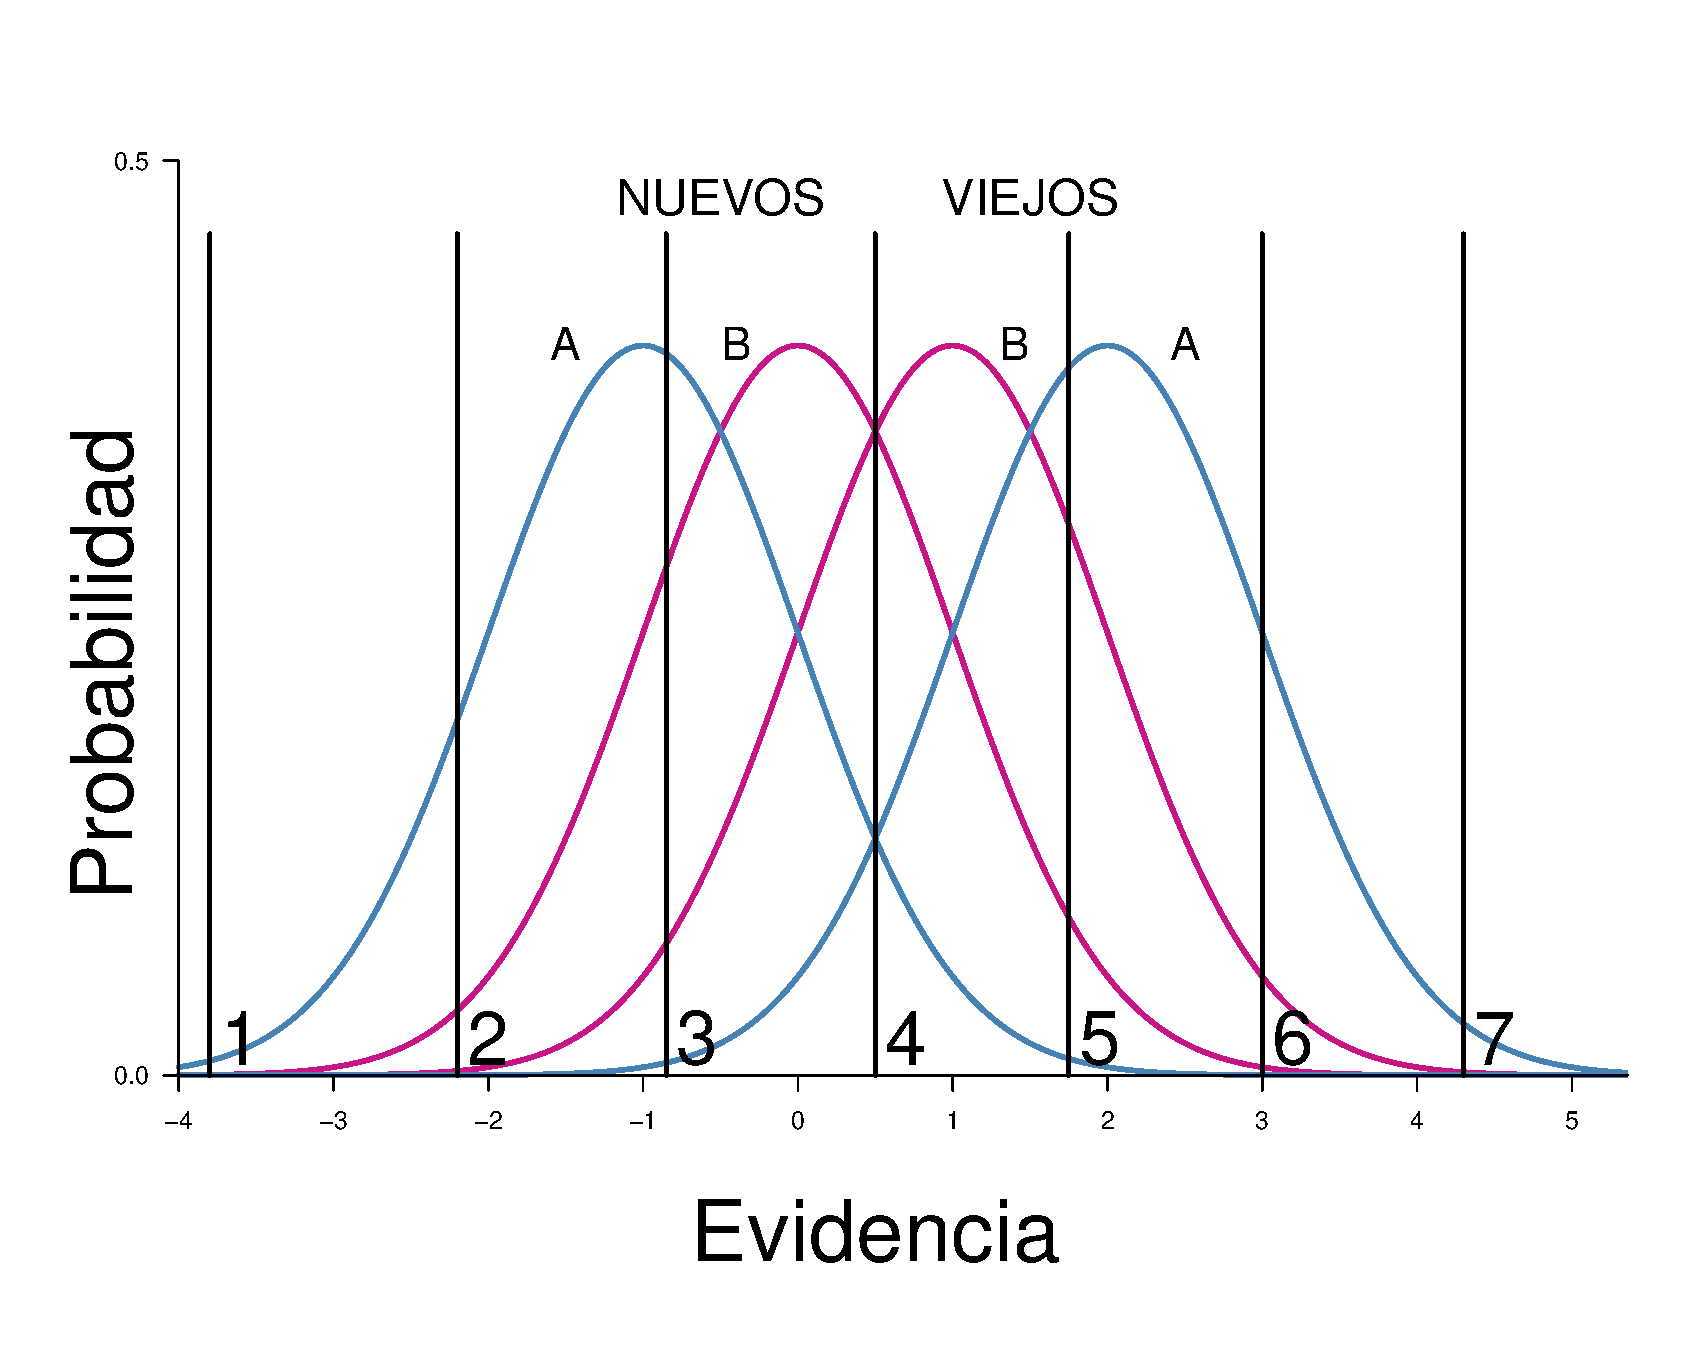
\includegraphics[width=0.7\textwidth]{Figures/EfectoEspejo_Puntajes}
%\decoRule
\caption[Representación gráfica de los sub-Criterios para la emisión de puntajes de confianza ]{}
\label{fig:Ejem_Efecto_Punt}
\end{figure}

En la Figura~\ref{fig:Ejem_Efecto_Punt} se ilustra la noción de que la relación entre el promedio de los puntajes asignados a cada tipo de estímulo (Viejo o Nuevo x A o B), corresponde con lo que se esperaría de acuerdo al órden en que las cuatro distribuciones se despliegan sobre el eje de evidencia: en general, las distribución de estímulos Nuevos A abarca criterios más bajos que la distribución de estímulos Nuevos B, y lo mismo ocurre con las distribuciones de estímulos Viejos.\\

\item \underline{Efecto Espejo en Tareas de Elección forzada entre dos alternativas}\\

Como se mencionó previamente, en las Tareas de Elección forzada de $m$ Alternativas se presenta a los participantes un número $m$ de estímulos por cada ensayo, de los cuales $m-1$ van a contener sólo ruido y sólamente $1$, la señal.En el caso particular de los estudios en Memoria de Reconocimiento que proporcionan evidencia sobre la prevalencia y consistencia del Efecto Espejo, se refieren experimentos que implementan tareas de Elección Forzada de dos alternativas donde en cada ensayo se presenta a los participantes una pareja conformadas por uno de los posibles estímulos con señal ($ViejoA$ o $ViejoB$) y uno de los dos tipos de ruido ($NuevoA$ o $NuevoB$), dejándoles la tarea de elegir cuál de los dos estímulos presentados en cada pareja fue presentado con anterioridad. En otras palabras, en este tipo de estudios se consideran cuatro posibles parejas de estímulos a presentar a los participantes en cada ensayo, identificadas como "parejas de comparación estándar":\\

\begin{itemize}
\item Señal A VS Ruido A  (ó Viejo A VS Nuevo A)\\
\item Señal A VS Ruido B (ó Viejo A VS Nuevo B)\\
\item Señal B VS Ruido A (ó Viejo B VS Nuevo A)\\
\item Señal B VS Ruido B (ó Viejo B VS Nuevo B)\\
\end{itemize}

En tareas de elección forzada entre dos alternativas, donde las parejas de estímulos presentados están compuestos por estímulos nuevos y viejos de dos clases distintas A y B, la evidencia en favor del Efecto Espejo aparece de la siguiente forma:\\

\begin{center}
$P(ViejoB, NuevoB) < P(ViejoB,NuevoA)$\\
y\\
$P(ViejoA, NuevoB) < P(ViejoA,NuevoA)$\\
\end{center}
\begin{center}
donde $P$ implica la proporción de veces que el primer elemento del paréntesis es elegido sobre del segundo, en tareas de elección forzada donde se solicita a los participantes que elijanel estímulo que les haya sido presentado con anterioridad, \parencite{Glanzer1993}.\\
\end{center}

En la interpretación de los datos obtenidos en este tipo de tareas, se asume que los participantes responden en cada ensayo eligiendo el estímulo con el valor más alto en términos de su ubicación en el eje de decisión. A su vez, en las parejas de comparación estándar formadas en experimentos que presentan evidencia en favor del Efecto Espejo, se asume que en cada ensayo los participantes comparan un estímulo proveniente de algunas de las distribuciones estímulos Viejos con un estímulo proveniente de alguna de las distribuciones de estímulos Nuevos. Tomando en cuenta la representación gráfica presentada en la Figura~\ref{fig:Ejem_EfectoEspejo}, podemos afirmar que existe una mayor distancia entre la distribución de estímulos Nuevos A (la distribución más orientada hacia el extremo izquierdo) y cualquiera de las distribuciones de estímulos Viejos A ó B, que entre cualquiera de estas y la distribución de estímulos Nuevos B (la segunda distribución presentada de izquierda a derecha). Es así que el patrón de respuestas encontrado en este tipo de estudios hace sentido a la luz del orden en que se despliegan las cuatro distribuciones subyacentes: en general, los participantes aciertan en mayor proporción (eligiendo el estímulo Viejo de la pareja) en las parejas donde el estímulo nuevo presentado pertenece a la clase A, ya que la distribución de donde estos  son extraídos se encuentra más alejada de las dos distribuciones de estímulos Viejos.\\

Como un control adicional, en este tipo de experimentos también se incluyen dos parejas adicionales, denominadas "parejas de comparación nula", compuestas por un mismo tipo de estímulo de cada clase:\\

\begin{itemize}
\item Señal A VS Señal B (ó ViejoA VS ViejoB)\\
\item Ruido A VS Ruido B (ó NuevoA VS NuevoB)\\
\end{itemize}

Mientras que en las parejas de comparación estándar las elecciones observadas en los participantes se interpretan en términos de las distancias entre las distribuciones de estímulos Viejos y cada distribución de estímulos Nuevos, las parejas de comparación nula proporcionan información acerca de la separación entre las distribuciones A y B de cada tipo de estímulo (Nuevo y Viejo). Si el orden de las cuatro distribuciones presentado como Efecto Espejo se sostiene, se espera encontrar que:\\

\begin{center}
$P(ViejoA, ViejoB) > 0.5$\\
y\\
$P(NuevoB, NuevoA) > 0.5$\\
\end{center}
\begin{center}
donde nuevamente $P$ representa la proporción de veces que se elige el primer elemento de cada paréntesis como aquel que fue presentado anteriormente y $0.5$ corresponde con la proporción esperada de acuerdo al azar, o bien, si asumiéramos que los participantes están eligiendo de manera aleatoria, \parencite{Glanzer1993}.\\ 
\end{center}

La idea detrás de la interpretación de las elecciones observadas en las parejas de comparación nula es que estas están compuestas por elementos que simultáneamente contienen, o no, la señal a detectar. Por ejemplo, en el caso de las parejas de comparación nula compuestas por dos estímulos Nuevos (uno de la clase A y uno B) no parece haber una razón por la cual los participantes deberían inclinarse a elegir uno en particular, y al final, la proporción de veces que se elige una clase de estímulo Nuevo sobre la otra debería acercarse al azar ($0.5$). Sin embargo, si es cierto que las cuatro distribuciones que subyacen a la presentación de estímulos A y B nuevos y viejos se presentan como sugiere el Efecto Espejo, se esperaría que a pesar de que cada pareja de comparación nula están compuestas por dos estímulos que corresponden con un mismo juicio de Reconocimiento, se elijan aquellos que se sitúen sobre los valores más altos del eje de evidencia. Es decir, si la distribución de estímulos Nuevos B se encuentra por encima de la distribución de estímulos Nuevos A y produce valores mayores de evidencia o "familiaridad", se espera que los participantes elijan los estímulos Nuevos B en una proporción de veces mayores al azar. La misma lógica es aplicada a las parejas de comparación nula compuestas por dos estímulos Viejos de distinta clase, \parencite{Glanzer1993}.\\

\end{itemize}

En un inicio, los patrones de respuestas actualmente identificados como parte del Efecto Espejo fueron conocidos como Efecto de Frecuencia de las Palabras \parencite{Schulman1967}, ya que fueron reportados por primera vez en estudios donde el desempeño de los participantes en tareas de reconocimiento se comparaba a través de dos clases de estímulos compuestas por palabras "poco comúnes" y palabras "muy comunes" de acuerdo a la Frecuencia de su uso \parencite{Kucera1967}. En dichos estudios, realizados con diferentes protocolos experimentales \parencite{Glanzer1976, Bowles1983, Glanzer1990}, se ha mostrado consistentemente evidencia de que las palabras poco comúnes eran reconocidas con mayor precisión tanto como "nuevas" como "viejas" (clase A) y que las palabras comúnes se confundían con mayor facilidad (clase B). No fue hasta que se demostró que estos mismos patrones de respuesta aparecían en cualquier tipo de tareas de reconocimiento en que se presentara a los participantes más de una clase de estímulos que se distinguieran entre sí por la precisión con que sus elementos son reconocidos en la fase de reconocimiento, sea cual sea la naturaleza de estas clases, que se comenzó a hablar del Efecto Espejo como una regularidad propia de la Memoria de Reconocimiento, \parencite{Allen1968, Glanzer1993}.\\

La evidencia del Efecto Espejo se presenta en una amplia variedad de estudios donde se manipulan distintas variables en la definición de las clases de estímulos A y B,  tales como la complejidad, la ortografía o la veracidad de los enunciados presentados. O bien, cuando se presentan grupos distintos de estímulos que se sabe son reconocidos con distinta precisión, por ejemplo, en estudios donde se comparan palabras con significado concreto (A) vs abstracto (B); imágenes (B) vs palabras (A); rostros comúnes (B) vs rostros poco comúnes (A), \parencite{Glanzer1993, Greene1996, Glanzer1998}.\\

\subsection{Relevancia, implicaciones e interpretaciones}\\

A primera vista el patrón de respuestas identificado como Efecto Espejo podría parecer trivial: si sabemos que lo que distingue a los grupos de estímulos A y B presentados en este tipo de estudios es la precisión con que sus elementos son reconocidos al presentarse más de una vez -o bien, que en una condición los elementos previamente vistos se vuelven más reconocibles que en la otra- tiene sentido esperar que los participantes tengan un mejor desempeño general (más aciertos y menos errores) en la clase A que en la clase B. Sin embargo, en el contexto específico de los estudios de Memoria de Reconicimiento, no parece claro por qué deberían haber diferencias entre las Falsas Alarmas registradas para cada clase de estímulo, en tanto que se trata de elementos que no han sido presentados antes y deberían de resultar igualmente "familiares" o "desconocidos".\\

Existen dos grandes formas en que el Efecto Espejo ha sido tratado en la literatura de Memoria de Reconocimiento:\\

\begin{numerate}
\item Como reflejo de los procesos cognitivos que subyacen a la ejecución de los participantes en las tareas de reconocimiento (tanto en la fase de estudio, como en la fase de reconocimiento).\\

\item Como evidencia de que el modelo de detección de señales no describe de manera adecuada el fenómeno de la Memoria de Reconocimiento.\\
\end{numerate}

Dentro de los modelos y teorías desarrollados para dar cuenta de lo que el Efecto Espejo podría estar sugiriendo acerca de la Memoria de Reconocimiento se pueden distinguir distintas aproximaciones.\\

Una primera aproximación para explicar el Efecto Espejo -y probablemente la más sencilla de todas- apela a las estrategias de respuesta empleadas por los participantes. Este tipo de explicaciones se sustentan en el hecho de que las discrepancias entre las tasas de Falsas Alarmas desaparecen cuando se solicita explícitamente a los participantes que "no adivinen" su respuesta \parencite{Greene1996}. Por ejemplo, la hipótesis de Distribución de las Respuestas \parencite{Greene1996}, supone que los participantes asumen por default que la cantidad de estímulos Viejos y Nuevos a presentarse durante el experimento es la misma y modulan deliberadamente la cantidad de respuestas afirmativas emitidas. Este tipo de explicaciones implican también que los participantes distinguen entre las dos clases de estímulos presentadas. De esta forma, dado que los participantes pueden identificar con mayor precisión los elementos "viejos" de la clase A ($Hits(A) > Hits(B)$) y emiten una mayor cantidad de respuestas afirmativas, cuando se les presentan estímulos nuevos de esta misma categoría son más estrictos al responder afirmativamente y reducen en consecuencia su tasa de falsas alarmas ($F.Alarmas(A) > F.Alarmas(B)$).\\

Un problema evidente con esta primera aproximación es que viola uno de los elementos clave detrás de la interpretación del Efecto Espejo como una fenómeno significativo y consistente en Memoria de Reconocimiento: el supuesto de que los participantes responden a partir de un sólo conjunto de criterios de elección que utilizan indistintamente entre las clases A y B. En otras palabras, este tipo de explicaciones sólo resultan válidas en experimentos donde las clases A y B son fáciles de distinguir entre sí y deja fuera el resto de los experimentos en que se ha encontrado evidencia del Efecto Espejo sin que los participantes sepan que su desempeño será comparado entre más de una condición, \parencite{Glanzer1998}.\\

Una segunda aproximación implica asumir que las clases de estímulos empleadas en estos estudios difieren en el efecto que tienen sobre los procesos superiores involucrados en las tareas de reconocimiento. En otras palabras, este segundo conjunto de explicaciones asume que cada clase de estímulos A y B es procesada de manera diferencial por el participante. Como uno de los ejemplos más representativos de este tipo de explicaciones se encuentra la Teoría de Atención/Verosimilitud \parencite{Glanzer1993}. Dicha teoría funciona como un modelo de muestreo de rasgos que se asume que todos los estímulos a presentar están compuestos por un número fijo de rasgos ($N$), de los cuales, algunos se presentan "marcados" desde su primera aparición como "rasgos familiares" ($p(new)$) y otros son marcados como tales una vez que se interactúa con ellos ($p(new) + [\alpha(i)* (1-p(new))]$). Esta teoría asume que la diferencia fundamental entre  las clases de estímulos probadas ($i$) es que elicitan distintos gradientes de atención que van a repercutir en el número de rasgos atendidos por los participantes ($n(i)$) dentro de $N$, definiendo una tasa de  "marcaje" propia de cada clase ($\alpha(i)$).\\

En otras palabras, el proceso mediante el cual se explica el Efecto Espejo de acuerdo a la Teoría de Atención/Verosimilitud es el siguiente:\\

\begin{enumerate}
\item Todos los estímulos están compuestos por una cantidad $N$ de rasgos que pueden o no estar marcados como "conocidos".\\

\item Todos los estímulos comienzan con una cierta proporción de rasgos marcados.\\
\begin{center}
$p(A,nuevo) = p(new)$\\
$p(B,nuevo) = p(new)$\\
Según el modelo, la cantidad de rasgos marcados inicialmente es la misma entre las clases A y B.\\
\end{center}

\item A y B difieren en el número de rasgos que los participantes muestrean al interactuar con cada estímulo.\\
\begin{center}
$n(A) > n(B)$\\
La clase A es más atendida que B.\\
\end{center}

\item De acuerdo con $n(i)$, A y B tienen su propia tasa de muestreo.\\
\begin{center}
$\alpha(A) = \frac{n(A)}{N}$\\
$\alpha(B) = \frac{n(B)}{N}$\\
donde si $n(A) > n(B)$ entonces, $\alpha(A) > \alpha(B)$\
\end{center}

\item Al interactuar con los estímulos presentados en la fase de estudio, los participantes muestrean cierto número de rasgos y marcan aquellos que no lo estén con anterioridad, ($\alpha(i)*(1-p(new))$).\\

\item En la fase de reconocimiento, los estímulos presentados previamente tienen una mayor proporción de rasgos marcados que los estímulos nuevos:\\
\begin{center}
$p(A,viejo) = p(new) + [\alpha(A)*(1-p(new))]$\\
$p(B,viejo) = p (new) + [\alpha(B)*(1-p(new))]$\\
\end{center}
\end{enumerate}

De acuerdo con la Teoría de Atención/Verosimilitud, los participantes registran sus respuestas en la fase de reconocimiento con base en la cantidad de rasgos "marcados" muestreado ($x$). La probabilidad de observar cierto valor de $x$ se describe en función a una distribución binomial con probabilidad $p(i,j)$ (donde $i$ es la clase A o B y $j$ es el tipo de estímulo: nuevo o viejos), para el total de observaciones $n(i)$ registradas en función a la clase del estímulo. Es decir:\\

\begin{center}
$p(x|p(i,j),n(i))$\\
\end{center}

Al observar una cantidad $x$ de rasgos marcados, los participantes emiten el juicio de reconocimiento que corresponda a dicha evidencia con mayor probabilidad, computando la razón de las verosimilitudes \parencite{Glanzer1993, Hintzman1994, Glanzer2009, Hilford2015}. De acuerdo con esta teoría, el Efecto Espejo se explica por medio de la siguiente relación:\\

\begin{center}
$p(x|p(A,nuevo),n(A)) < p(x|p(B,nuevo),n(B)) < p(x|p(B,viejo),n(B)) < p(x|p(A,viejo),n(A))$\\
\end{center}

En la Teoría de Atención/Verosimilitud el elemento clave para explicar las diferencias en el desempeño de los participantes entre A y B es la atención elicitada por cada clase y el número de rasgos muestreados en consecuencia ($n(i)$). Esto resuelve el problema de las discrepancias entre las tasas de Falsas Alarmas de la siguiente forma: aunque A y B contienen el mismo número de rasgos marcados en su primera presentación ($p(A,nuevo) = p(B,nuevo)$), el número de elementos muestreados es mayor en la condición A ($n(A) > n(B)$) y por tanto, hay una mayor probabilidad de extraer más rasgos marcados que en B ($p(x|p(A,nuevo),n(A)) < p(x|p(B,nuevo),n(B))$).\\

Pese al conjunto de experimentos desarrollados para probar la solidez de la Teoría de Atención/Verosimilitud mediante la manipulación de distintas variables experimentales que deberian tener un impacto sobre los parámetros del modelo (por ejemplo, restringiendo el tiempo de estudio y/o de respuesta para modificar $n(i)$ en cada fase) y evaluando la precisión con que el modelo predice y explica los datos encontrados, \parencite{Glanzer1993, Kim1993, Glanzer1991}, la Teoría de Atención/Verosimilitud ha sido fuertemente criticada en relación a dos grandes factores: 1) la teoría está compuesta por parámetros y supuestos innecesariamente complejos que le restan validez ecológica y 2) la teoría asume que los participantes tienen acceso a información completa sobre la estructura de la tarea y son capaces de utilizarla para realizar cómputos altamente demandantes, \parencite{Hintzman1994, Murdock1998, DeCarlo2007}.\\

Una tercera forma de interpretar el Efecto Espejo es de manera consistente con la aplicación de la TDS al análisis de las tareas de reconocimiento: asumiendo que los participantes registran sus respuestas en función a la evidencia que evalúan en cada ensayo (la "fuerza de memoria" o "familiaridad" contenida en el eje de evidencia), sin necesidad de recurrir a ningún tipo de cómputo adicional \parencite{Hintzman1994}. Bajo esta perspectiva, la única diferencia que existe entre las clases A y B -sin importar si pueda justificarse el por qué de ella- es la "fuerza de memoria" que contienen, o bien qué tan familiares resultan para los participantes. Por ejemplo, en los estudios donde se usan distintos niveles de "Palabras frecuentes" para delimitar las clases de estímulos a comparar, las palabras poco comúnes parecen ser más fáciles de recordar y reconocer (A) y las palabras comúnes parecen confundirse con mayor facilidad (B). De acuerdo a este tipo de explicaciones, las palabras comúnes Nuevas (B,Nuevo) tienen un mayor grado de familiaridad que los estímulos Nuevos poco comúnes (A,Nuevo), por lo que la separación de las dos distribuciones de estímulos Nuevos tiene sentido. A su vez, dado que las palabras poco comúnes son más salientes, se asume que se les presta más atención y terminan adquiriendo un mayor nivel de familiaridad cuando se les presenta por segunda vez que las palabras comúnes, lo que termina explicando el orden en que se presentan las distribuciones de estímulos Viejos, \parencite{Glanzer1993}.\\

En una dirección distinta, se encuentran las interpretaciones del Efecto Espejo que tienden a tomarle como evidencia para desacreditar el uso de la TDS para estudiar del fenómeno de la memoria de reconocimiento. Por ejemplo, un primer conflicto evidente en la interpretación del Efecto Espejo es que no siempre parece claro por qué una de las clases de estímulos a probar debería resultar "más familiar" (A) que la otra (B) desde que se presenta en la fase de estudio. Aún cuando este tipo de explicaciones se sostiene de manera intuitiva para entender los resultados encontrados en estudios donde A y B se componen de palabras poco comúnes y comúnes, cuando se intenta añadir una tercer clase C, compuesta por palabras "raras", los resultados encontrados no son consistentes con lo que la interpretación del Efecto Espejo sugeriría,  \parencite{Rao1984, Wixted1992}. En general, se esperaría que la nueva clase C añadiera dos distribuciones más sobre el eje de evidencia, que se agregarían hacia los extremos inferior y superior del mismo. Sin embargo, este no parece ser el caso.\\

Por último, como un punto intermedio se encuentran los trabajos orientados al desarrollo y evaluación de distintos modelos de detección de señales que, aunque parten de los supuestos principales de la TDS, difieren en un sentido más formal, en la naturaleza que se asume tienen las distribuciones subyacentes a la tarea. Por ejemplo, asumiendo distintos tipos de distribuciones \parencite{Glanzer1993, Glanzer2009} o bien, fomentando el abordaje del problema desde la perspectiva de los modelos de mezclas en detección de señales, \parencite{DeCarlo2002, DeCarlo2007}.\\

\section{Planteamiento del problema}

Tal y como se describió en la sección anterior, el Efecto Espejo es un fenómeno empírico reportado de manera consistente en diversos estudios de Memoria de Reconocimiento abordados bajo el marco de la TDS. Dicho fenómeno ha sido motivo de cierto revuelo en la literatura en Memoria, impulsando el desarrollo de distintos tipos de explicaciones, modelos y teorías orientados a dar cuenta de su ocurrencia, tanto en términos de lo que podría estar sugiriendo acerca de cómo opera la Memoria de Reconocimiento, como del desarrollo de nuevas variantes del modelo de detección de señales que permitan una mejor descripción del desempeño de los participantes en este tipo de tareas a la luz de las respuestas observadas.\\

Más allá de la amplia variedad -tanto en complejidad como en su naturaleza- de propuestas desarrolladas para dar cuenta del Efecto Espejo como un fenómeno intrínseco de la Memoria de Reconocimiento, se resalta el hecho de que este fenómeno no ha sido estudiado ni reportado en ningún estudio donde el marco de la TDS sea aplicado a algún otro fenómeno o tarea de detección. La evaluación de la generalizabilidad del Efecto Espejo a otras áreas de aplicación de la TDS se considera relevante en tanto que 1) provería un contexto más amplio para interpretar el Efecto Espejo como resultado "estándar" en toda tarea de detección donde el desempeño de los participantes se compare entre dos niveles de $d'$ y no sólo como un fenómeno particular de la Memoria de Reconocimiento (o viceversa); y 2) de observarse evidencia del Efecto Espejo en otro tipo de tareas de detección, la pertinencia de la aplicación del modelo de la TDS al estudio específico de la memoria de reconocimiento podría ser evaluada con mayor claridad en función a lo que dicho patrón de respuestas podría estar sugiriendo -en general- sobre el problema de la detección bajo incertidumbre, con independencia del área específica en que estos se sitúen.\\

El trabajo de tesis aquí presentado no se ocupa de revisar ni de evaluar en forma alguna las propuestas teóricas y formales desarrolladas para dar cuenta del Efecto Espejo como un fenómeno inherente a la Memoria de Reconocimiento. El objetivo del trabajo de investigación realizado es el de evaluar la existencia de los patrones de respuesta identificados como Efecto Espejo en una tarea de detección desarrollada fuera del marco conceptual de la Memoria de Reconocimiento. Para ello, se propuso trabajar con una tarea de detección meramente perceptual con dos clases de estímulos A y B que difieren en su discriminabilidad y que fueron construidas con base en lo que se ha reportado en la literatura.\\

